\documentclass[conference]{IEEEtran}
\IEEEoverridecommandlockouts

\usepackage{cite}
\usepackage{amsmath,amssymb,amsfonts}
\usepackage{algorithmic}
\usepackage{graphicx}
\usepackage{textcomp}
\usepackage{xcolor}
\usepackage{array}
\usepackage{booktabs}

\graphicspath{{images/}}

\def\BibTeX{{\rm B\kern-.05em{\sc i\kern-.025em b}\kern-.08em
    T\kern-.1667em\lower.7ex\hbox{E}\kern-.125emX}}

\begin{document}

\title{A Data Lens on Crime in LA:\\LA Crime Analytics 2020--Present}

\author{
\IEEEauthorblockN{Samuel Winkens}
\IEEEauthorblockA{\textit{Department of Computer Science}\\
\textit{University at Buffalo}\\
Buffalo, NY\\
sdwinken@buffalo.edu}
\and
\IEEEauthorblockN{Mansur Nafis}
\IEEEauthorblockA{\textit{Department of Computer Science}\\
\textit{University at Buffalo}\\
Buffalo, NY\\
mansurna@buffalo.edu}
}

\maketitle

\begin{abstract}
Los Angeles generates thousands of crime reports annually, yet the raw data published by the Los Angeles Police Department (LAPD) lacks structure, making it difficult for residents, law enforcement, and government agencies to extract meaningful insights. This paper presents the design and implementation of a normalized relational database---LA Crime Analytics 2020-Present---that transforms unstructured LAPD crime data into a queryable, consistent schema. The database organizes data into nine tables covering crime reports, occurrence timing, geographic locations, victim demographics, crime classifications, weapon types, premise types, and case statuses. We describe the entity-relationship model, full table definitions, and a suite of SQL queries, stored procedures, user-defined functions, transactions, and index optimizations that demonstrate the system's analytical capabilities. Index-based optimizations yielded query cost reductions of over 99\% in two of three tested scenarios.
\end{abstract}

\begin{IEEEkeywords}
relational database, crime analytics, LAPD, SQL, normalization, indexing, PostgreSQL
\end{IEEEkeywords}

% ---------------------------------------------------------------
\section{Introduction}

Los Angeles is one of the most densely populated and crime-affected cities in the world. It generates thousands of crime reports every year; however, the data published by the LAPD has no inherent structure---it appears as an unorganized collection of numbers and descriptors. This causes significant problems for those who wish to analyze the data. On a non-database solution, inquiries produce slow and inconsistent results. Filtering by key attributes such as area, victim demographics, premise type, or weapon type is cumbersome, and identifying trends is nearly impossible since the data is not in a queryable format.

These limitations affect multiple stakeholder groups. Law enforcement agencies struggle to identify crime patterns and deploy officers to the correct areas. Los Angeles city governments lack the structured data needed to justify funding allocations and build accurate public safety policies. Residents lack tools to assess neighborhood risk and make informed decisions about where to live, work, and travel.

Our database addresses these issues by designing and implementing a normalized relational database that structures LA crime data into clearly defined schemas. When a new report is submitted, all related data is consistently updated in accordance with the normalized schema, supporting real-time updates, structured attribute-based queries, and trend analysis across time.

% ---------------------------------------------------------------
\section{Problem Statement}

\subsection{Core Problems}
\begin{itemize}
    \item Los Angeles crime data is updated continuously, making it difficult to extract important information and trends from raw data.
    \item Given the sheer volume of data, ad-hoc queries are slow and can produce inconsistent results.
    \item The raw data is unsorted and unorganized, making it difficult to filter on specific criteria such as area, victim sex, weapon used, or crime method.
\end{itemize}

\subsection{Significance}
Crime data is used by residents to decide which routes to take and which neighborhoods to live in. Agencies and local government use it to allocate funding and drive policy decisions. Law enforcement uses it to predict where future crimes may occur and preemptively deploy resources.

\subsection{Proposed Solution}
Our project ensures that when new data is entered it is immediately available, guaranteeing consistency for historical queries as well as current ones. It enables residents, agencies, and local governments to query data by specific area and criteria within Los Angeles. Furthermore, the schema could be adopted by other cities to implement their own structured crime databases.

% ---------------------------------------------------------------
\section{Target Users}

The primary users of this database system include:
\begin{itemize}
    \item \textbf{Police Departments and City Agencies:} These users can analyze crime patterns to improve patrol planning, resource allocation, and policy decisions.
    \item \textbf{Los Angeles Residents:} Citizens can use the database to identify areas with higher crime rates and understand when certain crimes are more likely to occur.
\end{itemize}

\subsection{Administrative Roles}
Initially, a senior IT director for the LAPD would administer the database for LAPD crime data. If the schema is adopted by other cities, each city's police IT team would receive a copy of the database blueprint to generate their own instance. As adoption grows, a centralized organization could manage a unified national database spanning multiple cities.

\subsection{Usage Scenario}
Consider an officer who reports a theft in North Hollywood. Upon submission, the report is converted to fit the LA Crime database schema and is immediately visible to all authorized users. Later that day, a detective notices an increase in criminal activity in North Hollywood. By querying the database by area, time, and crime type, the detective discovers that thefts are spiking from 6--7~PM on weekends. Patrolmen are deployed during those hours, local businesses are warned, and residents are informed to avoid the area at those times. This illustrates how a single incident, properly stored in a structured database, can benefit law enforcement, businesses, and civilians simultaneously.

% ---------------------------------------------------------------
\section{Database Design}

\subsection{Entity-Relationship Diagram}

The entity-relationship (E/R) diagram for the LA Crime Analytics database is shown in Fig.~\ref{fig:er}. The diagram was created using Lucidchart~\cite{lucidchart}.

\begin{figure}[htbp]
\centerline{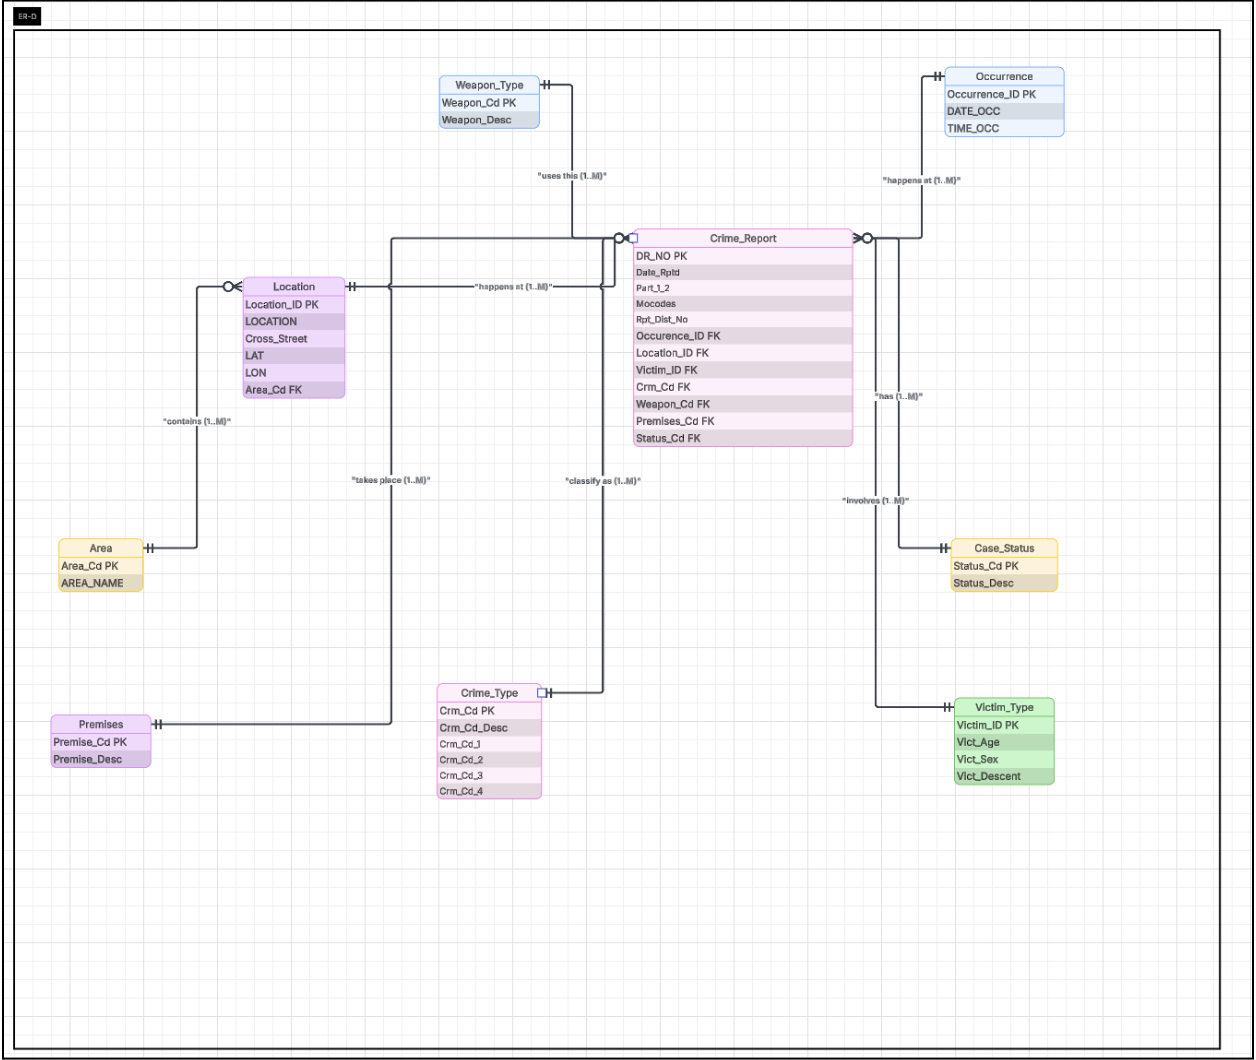
\includegraphics[width=\columnwidth]{er-diagram.png}}
\caption{Entity-Relationship diagram for the LA Crime Analytics database.}
\label{fig:er}
\end{figure}

\subsection{Relations and Attributes}

The database comprises nine relations. Primary keys and foreign keys are identified for each relation, followed by detailed attribute definitions. All attribute names were drawn directly from the LAPD dataset column names where applicable.

\subsubsection{Crime\_Report}

\textbf{Primary Key:} \texttt{DR\_NO} (bigint) --- uniquely identifies each crime report so every record can be referenced and connected to related data.

\textbf{Foreign Keys:} \texttt{Occurrence\_ID}, \texttt{Location\_ID}, \texttt{Victim\_ID}, \texttt{Crm\_Cd}, \texttt{Weapon\_Cd}, \texttt{Premise\_Cd}, \texttt{Status\_Cd}.

Table~\ref{tab:crime_report} lists the full attribute definitions for \texttt{Crime\_Report}.

\begin{table*}[htbp]
\caption{Crime\_Report Attribute Definitions}
\label{tab:crime_report}
\begin{center}
\footnotesize
\begin{tabular}{|p{2cm}|p{2cm}|p{0.7cm}|p{6.5cm}|p{1.8cm}|p{1.8cm}|}
\hline
\textbf{Attribute} & \textbf{Data Type} & \textbf{Key} & \textbf{Description / Purpose} & \textbf{Default Value} & \textbf{Delete Action} \\
\hline
DR\_NO & bigint & PK & Unique identifier for each crime report. Allows every report to be uniquely referenced and connected to related data. & NOT NULL & --- \\
\hline
Date\_Rptd & date & --- & Date the incident was officially reported. Distinguishes the reporting date from the actual occurrence date. & NOT NULL & --- \\
\hline
Part\_1\_2 & int & --- & Indicates Part 1 or Part 2 crime classification. Useful for grouping and analyzing offense severity. & NULL & --- \\
\hline
Mocodes & varchar(100) & --- & Method-of-operation codes associated with the report. Preserves crime-pattern details used in analysis. Not critically required. & NULL & --- \\
\hline
Rpt\_Dist\_No & int & --- & Reporting district number for the crime report. Useful for geographic and police-district analysis. & NULL & --- \\
\hline
Occurrence\_ID & bigint & FK & Links the report to the Occurrence table so date/time occurrence data is not duplicated in every report row. & NOT NULL & Block Delete \\
\hline
Location\_ID & int & FK & Links the report to the Location table so location details are normalized and reusable across reports. & NOT NULL & Block Delete \\
\hline
Victim\_ID & int & FK & Links the report to Victim\_Type to associate the crime with victim demographic information. & NULL & Block Delete \\
\hline
Crm\_Cd & int & FK & Links the report to the primary crime classification in Crime\_Type. Avoids storing repeated crime descriptions in every report. & NOT NULL & Block Delete \\
\hline
Weapon\_Cd & int & FK & Links the report to Weapon\_Type to identify the weapon involved, if any. & NULL & Block Delete \\
\hline
Premise\_Cd & int & FK & Links the report to Premises to identify the type of place where the incident occurred. & NOT NULL & Block Delete \\
\hline
Status\_Cd & char(2) & FK & Links the report to Case\_Status so the current case status is publicly known. & NOT NULL & Block Delete \\
\hline
\end{tabular}
\end{center}
\end{table*}

\subsubsection{Occurrence}

\textbf{Primary Key:} \texttt{Occurrence\_ID} (bigint). Every crime report has at least one occurrence, so this field cannot be null. Table~\ref{tab:occurrence} lists the attributes.

\begin{table}[htbp]
\caption{Occurrence Attribute Definitions}
\label{tab:occurrence}
\begin{center}
\footnotesize
\begin{tabular}{|p{1.6cm}|p{1cm}|p{0.5cm}|p{3.2cm}|p{1.2cm}|}
\hline
\textbf{Attribute} & \textbf{Type} & \textbf{Key} & \textbf{Description} & \textbf{Default} \\
\hline
Occurrence\_ID & bigint & PK & ID linking to Crime\_Report; identifies when each crime occurred. & NOT NULL \\
\hline
DATE\_OCC & date & --- & Date the crime occurred for this Occurrence\_ID. & NOT NULL \\
\hline
TIME\_OCC & int & --- & Time the crime occurred for this Occurrence\_ID. & NOT NULL \\
\hline
\end{tabular}
\end{center}
\end{table}

\subsubsection{Area}

\textbf{Primary Key:} \texttt{Area\_Cd} (int). Every crime must have an area where it happened. Table~\ref{tab:area} lists the attributes.

\begin{table}[htbp]
\caption{Area Attribute Definitions}
\label{tab:area}
\begin{center}
\footnotesize
\begin{tabular}{|p{1.6cm}|p{1.3cm}|p{0.5cm}|p{3.2cm}|p{1.2cm}|}
\hline
\textbf{Attribute} & \textbf{Type} & \textbf{Key} & \textbf{Description} & \textbf{Default} \\
\hline
Area\_Cd & int & PK & Unique area code associated with each area name. & NOT NULL \\
\hline
AREA\_NAME & varchar(100) & --- & Human-readable name associated with the area code. & NOT NULL \\
\hline
\end{tabular}
\end{center}
\end{table}

\subsubsection{Location}

\textbf{Primary Key:} \texttt{Location\_ID} (int). \textbf{Foreign Key:} \texttt{Area\_Cd}. Many locations can belong to one area. Table~\ref{tab:location} lists the attributes.

\begin{table}[htbp]
\caption{Location Attribute Definitions}
\label{tab:location}
\begin{center}
\footnotesize
\begin{tabular}{|p{1.6cm}|p{1.3cm}|p{0.5cm}|p{3.2cm}|p{1.2cm}|}
\hline
\textbf{Attribute} & \textbf{Type} & \textbf{Key} & \textbf{Description} & \textbf{Default} \\
\hline
Location\_ID & int & PK & Unique identifier for a location; allows reuse across multiple crime reports. & NOT NULL \\
\hline
LOCATION & varchar(100) & --- & Street address, block, or general location description. & NULL \\
\hline
Cross\_Street & varchar(100) & --- & Nearby cross street for improved geographic context. & NULL \\
\hline
LAT & float & --- & Latitude coordinate for map-based analysis and spatial queries. & NULL \\
\hline
LON & float & --- & Longitude coordinate for map-based analysis and spatial queries. & NULL \\
\hline
Area\_CD & int & FK & Links the location to its LAPD area (many locations to one area). & NOT NULL \\
\hline
\end{tabular}
\end{center}
\end{table}

\subsubsection{Victim\_Type}

\textbf{Primary Key:} \texttt{Victim\_ID} (int). Because exact victim identifiers (e.g., SSN) are unavailable, only demographic data is stored. Table~\ref{tab:victim} lists the attributes.

\begin{table}[htbp]
\caption{Victim\_Type Attribute Definitions}
\label{tab:victim}
\begin{center}
\footnotesize
\begin{tabular}{|p{1.6cm}|p{1.3cm}|p{0.5cm}|p{3.2cm}|p{1.2cm}|}
\hline
\textbf{Attribute} & \textbf{Type} & \textbf{Key} & \textbf{Description} & \textbf{Default} \\
\hline
Victim\_ID & int & PK & ID linking to Crime\_Report; key for the victim demographic record. & NOT NULL \\
\hline
Vict\_Age & int & --- & Age of the crime victim. & NULL \\
\hline
Vict\_Sex & varchar(1) & --- & Sex of the crime victim. & NULL \\
\hline
Vict\_Descent & varchar(1) & --- & Race/descent of the crime victim. & NULL \\
\hline
\end{tabular}
\end{center}
\end{table}

\subsubsection{Crime\_Type}

\textbf{Primary Key:} \texttt{Crm\_Cd} (int). Every crime report must have at least one crime type. Table~\ref{tab:crimetype} lists the attributes.

\begin{table}[htbp]
\caption{Crime\_Type Attribute Definitions}
\label{tab:crimetype}
\begin{center}
\footnotesize
\begin{tabular}{|p{1.6cm}|p{1.3cm}|p{0.5cm}|p{3.2cm}|p{1.2cm}|}
\hline
\textbf{Attribute} & \textbf{Type} & \textbf{Key} & \textbf{Description} & \textbf{Default} \\
\hline
Crm\_Cd & int & PK & Unique code identifying a crime classification used by Crime\_Report. & NOT NULL \\
\hline
Crm\_Cd\_Desc & text & --- & Human-readable description of the crime type; every crime must have one. & NOT NULL \\
\hline
Crm\_Cd\_1 & int & --- & Primary crime code; required for every crime. & NOT NULL \\
\hline
Crm\_Cd\_2 & int & --- & Optional secondary crime code for the same incident. & NULL \\
\hline
Crm\_Cd\_3 & int & --- & Optional tertiary crime code for the same incident. & NULL \\
\hline
Crm\_Cd\_4 & int & --- & Optional quaternary crime code for the same incident. & NULL \\
\hline
\end{tabular}
\end{center}
\end{table}

\subsubsection{Weapon\_Type}

\textbf{Primary Key:} \texttt{Weapon\_Cd} (int). A weapon entry may have a null description if no weapon was used. Table~\ref{tab:weapon} lists the attributes.

\begin{table}[htbp]
\caption{Weapon\_Type Attribute Definitions}
\label{tab:weapon}
\begin{center}
\footnotesize
\begin{tabular}{|p{1.6cm}|p{1.3cm}|p{0.5cm}|p{3.2cm}|p{1.2cm}|}
\hline
\textbf{Attribute} & \textbf{Type} & \textbf{Key} & \textbf{Description} & \textbf{Default} \\
\hline
Weapon\_Cd & int & PK & Unique code identifying the weapon type used in the crime. & NOT NULL \\
\hline
Weapon\_Desc & text & --- & Description of the weapon used, or empty if none was involved. & NULL \\
\hline
\end{tabular}
\end{center}
\end{table}

\subsubsection{Premises}

\textbf{Primary Key:} \texttt{Premise\_Cd} (int). Every crime report has a premise type because that is a mandatory field in LAPD reporting. Table~\ref{tab:premises} lists the attributes.

\begin{table}[htbp]
\caption{Premises Attribute Definitions}
\label{tab:premises}
\begin{center}
\footnotesize
\begin{tabular}{|p{1.6cm}|p{1.3cm}|p{0.5cm}|p{3.2cm}|p{1.2cm}|}
\hline
\textbf{Attribute} & \textbf{Type} & \textbf{Key} & \textbf{Description} & \textbf{Default} \\
\hline
Premise\_Cd & int & PK & Unique code identifying the premise type; referenced by Crime\_Report. & NOT NULL \\
\hline
Premise\_Desc & text & --- & Description of the premise (e.g., street, sidewalk, alley). & NOT NULL \\
\hline
\end{tabular}
\end{center}
\end{table}

\subsubsection{Case\_Status}

\textbf{Primary Key:} \texttt{Status\_Cd} (char(2)). Every crime must have a case status entered at the time of reporting. Table~\ref{tab:casestatus} lists the attributes.

\begin{table}[htbp]
\caption{Case\_Status Attribute Definitions}
\label{tab:casestatus}
\begin{center}
\footnotesize
\begin{tabular}{|p{1.6cm}|p{1.3cm}|p{0.5cm}|p{3.2cm}|p{1.2cm}|}
\hline
\textbf{Attribute} & \textbf{Type} & \textbf{Key} & \textbf{Description} & \textbf{Default} \\
\hline
Status\_Cd & char(2) & PK & Unique two-character code associated with one status description. & NOT NULL \\
\hline
Status\_Desc & varchar(100) & --- & Human-readable description of the current case status. & NOT NULL \\
\hline
\end{tabular}
\end{center}
\end{table}

\subsection{Defined Relationships}

The following many-to-one relationships are defined in the schema:
\begin{enumerate}
    \item Many \texttt{Crime\_Report} rows can reference the same \texttt{Occurrence} (date and time).
    \item Many \texttt{Crime\_Report} rows can reference the same \texttt{Location} (latitude, longitude, and area FK).
    \item Many \texttt{Crime\_Report} rows can reference the same \texttt{Victim\_Type} (since only demographic data, not unique identifiers, is stored).
    \item Many \texttt{Crime\_Report} rows can classify under the same \texttt{Crime\_Type}.
    \item Many \texttt{Crime\_Report} rows can involve the same \texttt{Weapon\_Type}.
    \item Many \texttt{Crime\_Report} rows can occur at the same \texttt{Premises} type.
    \item Many \texttt{Crime\_Report} rows can share the same \texttt{Case\_Status}.
    \item Many \texttt{Location} records can belong to one \texttt{Area}.
\end{enumerate}

% ---------------------------------------------------------------
\section{Phase 2: Implementation}

Phase 2 extended the database with data modification scripts, a stored procedure, a user-defined function, analytical select queries, a transaction with trigger-based validation, and index optimizations. No new assumptions, E/R diagram changes, or schema modifications were introduced.

\subsection{Contributions}

\textbf{Samuel:} Created the README, \texttt{create.sql}, \texttt{get\_crime\_count.sql}, \texttt{indexes.sql}, and \texttt{select\_queries.sql}.

\textbf{Mansur:} Created the seed-data generation script (\texttt{seed\_data.sql}), \texttt{data\_modifications.sql}, \texttt{transaction.sql}, and \texttt{gen\_test\_data.sql} (19 test rows).

\subsection{Data Modifications}

The data modification script inserts a new record into the \texttt{Crime\_Report} table. Fig.~\ref{fig:insert_query} shows the insert statement, and Fig.~\ref{fig:insert_output} confirms the successful insertion by displaying the stored row.

\begin{figure}[htbp]
\centerline{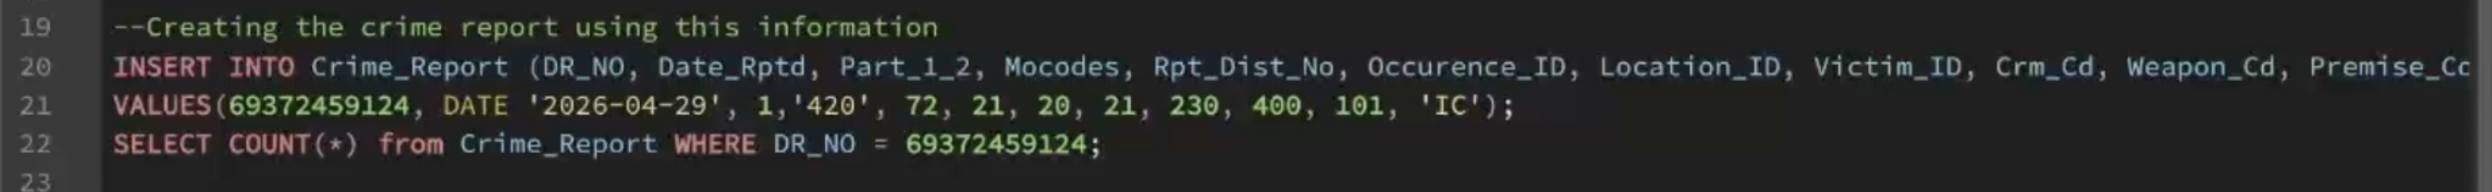
\includegraphics[width=\columnwidth]{phase2-insert-query.png}}
\caption{Insert statement adding a new crime report to the Crime\_Report table.}
\label{fig:insert_query}
\end{figure}

\begin{figure}[htbp]
\centerline{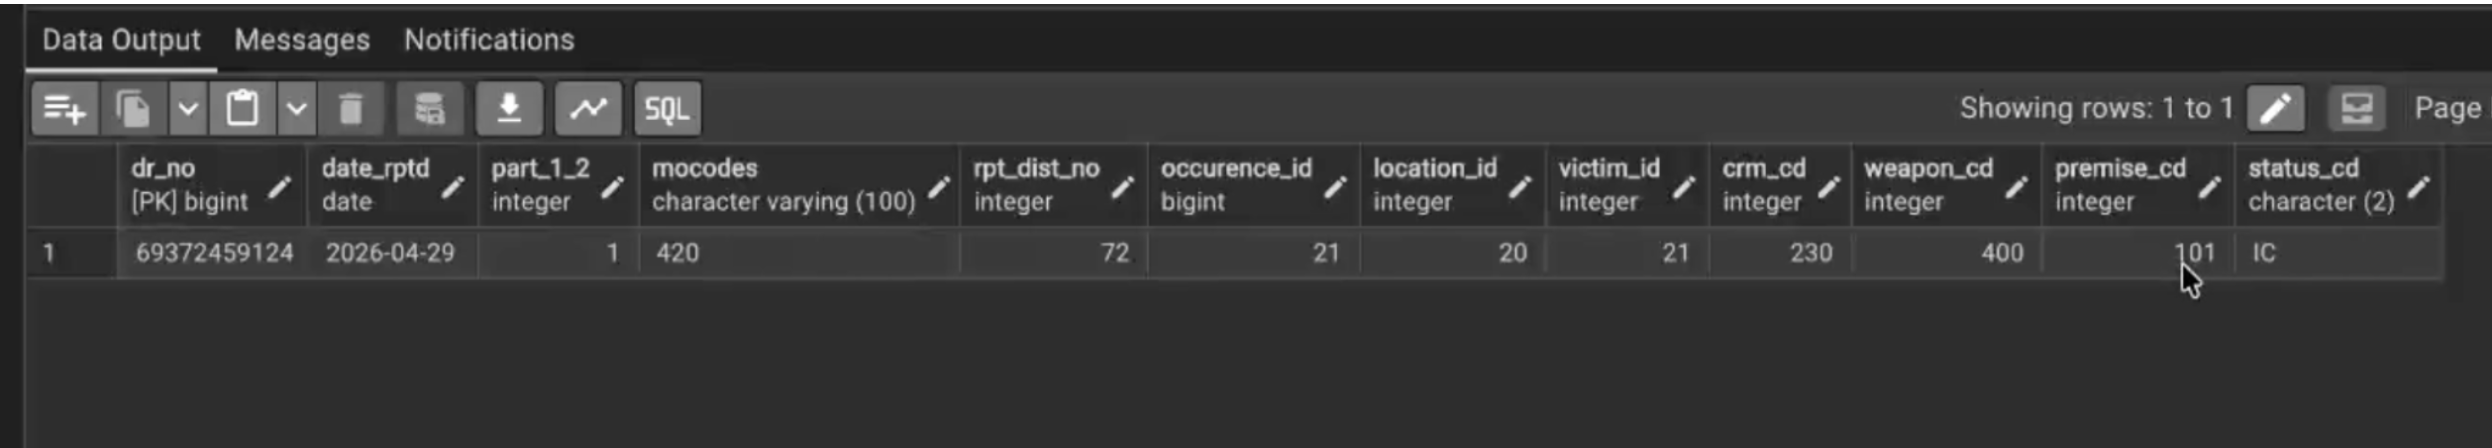
\includegraphics[width=\columnwidth]{phase2-insert-output.png}}
\caption{Output confirming the successful insertion of the new crime report.}
\label{fig:insert_output}
\end{figure}

\subsection{Stored Procedure}

The stored procedure accepts a \texttt{DR\_NO} (primary key in \texttt{Crime\_Report}) and a new status value as parameters. It updates the corresponding row in \texttt{Crime\_Report} with the new \texttt{Status\_Cd}. Fig.~\ref{fig:proc_query} shows the procedure definition, and Fig.~\ref{fig:proc_output} shows the record after execution, confirming the status change.

\begin{figure}[htbp]
\centerline{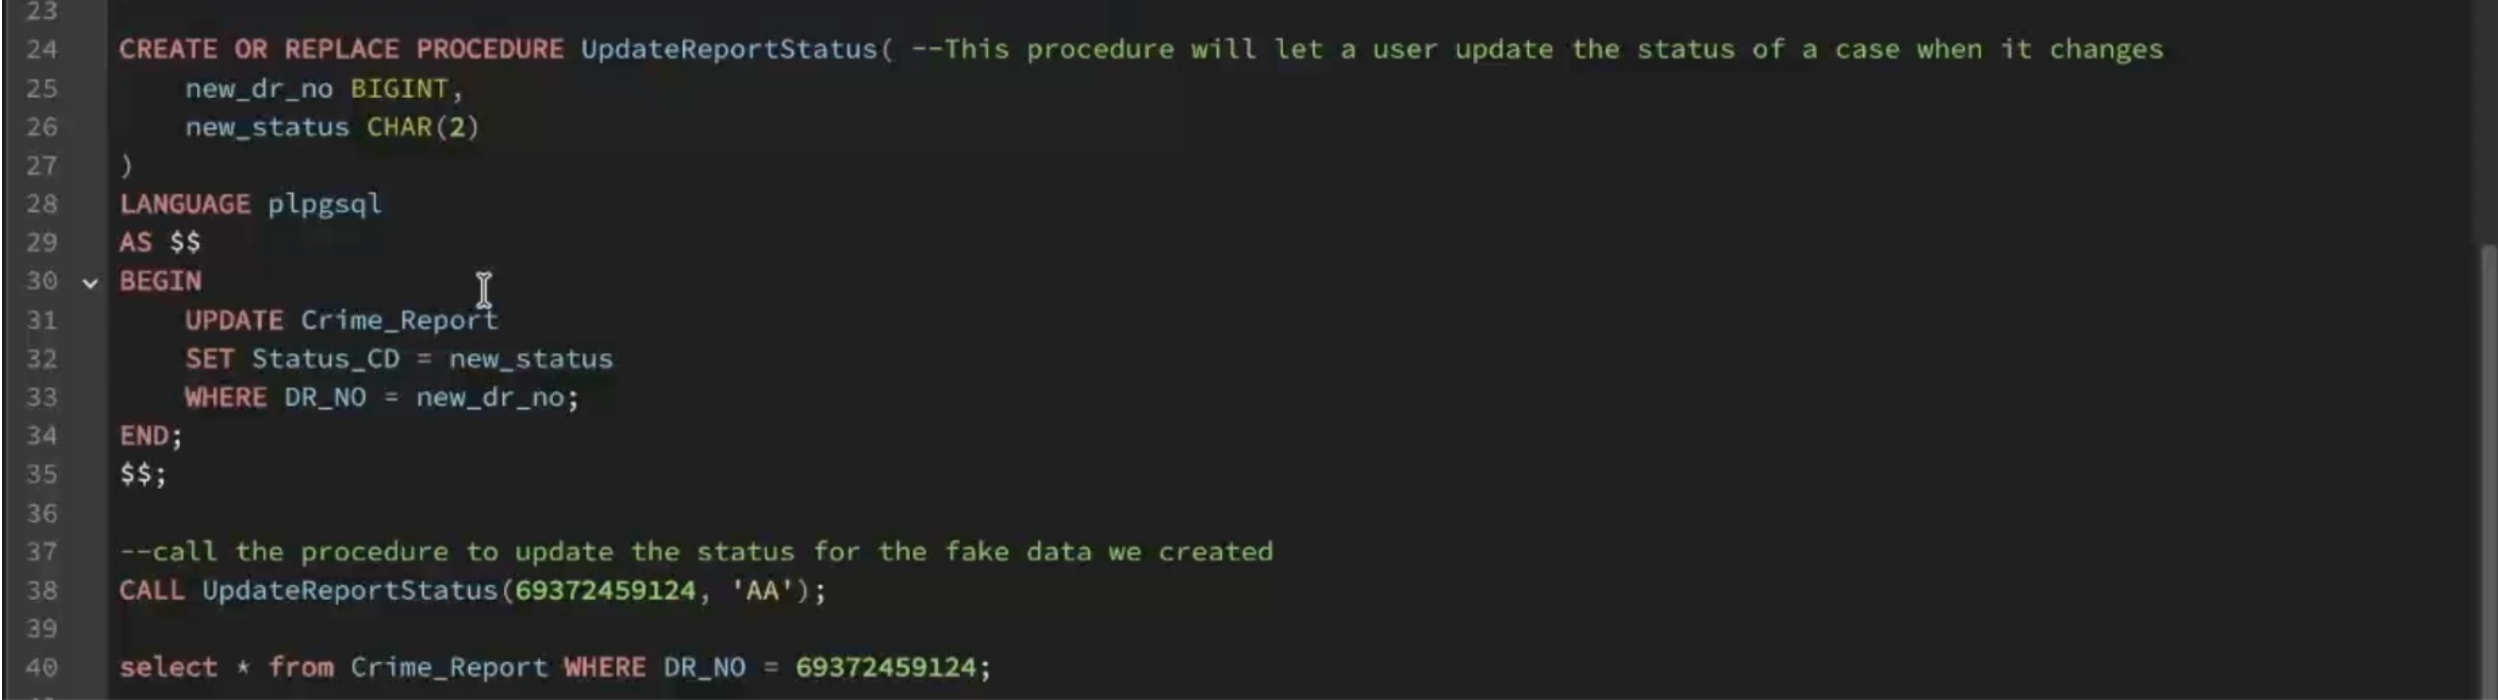
\includegraphics[width=\columnwidth]{procedure-query.png}}
\caption{Stored procedure definition for updating the status of a crime report.}
\label{fig:proc_query}
\end{figure}

\begin{figure}[htbp]
\centerline{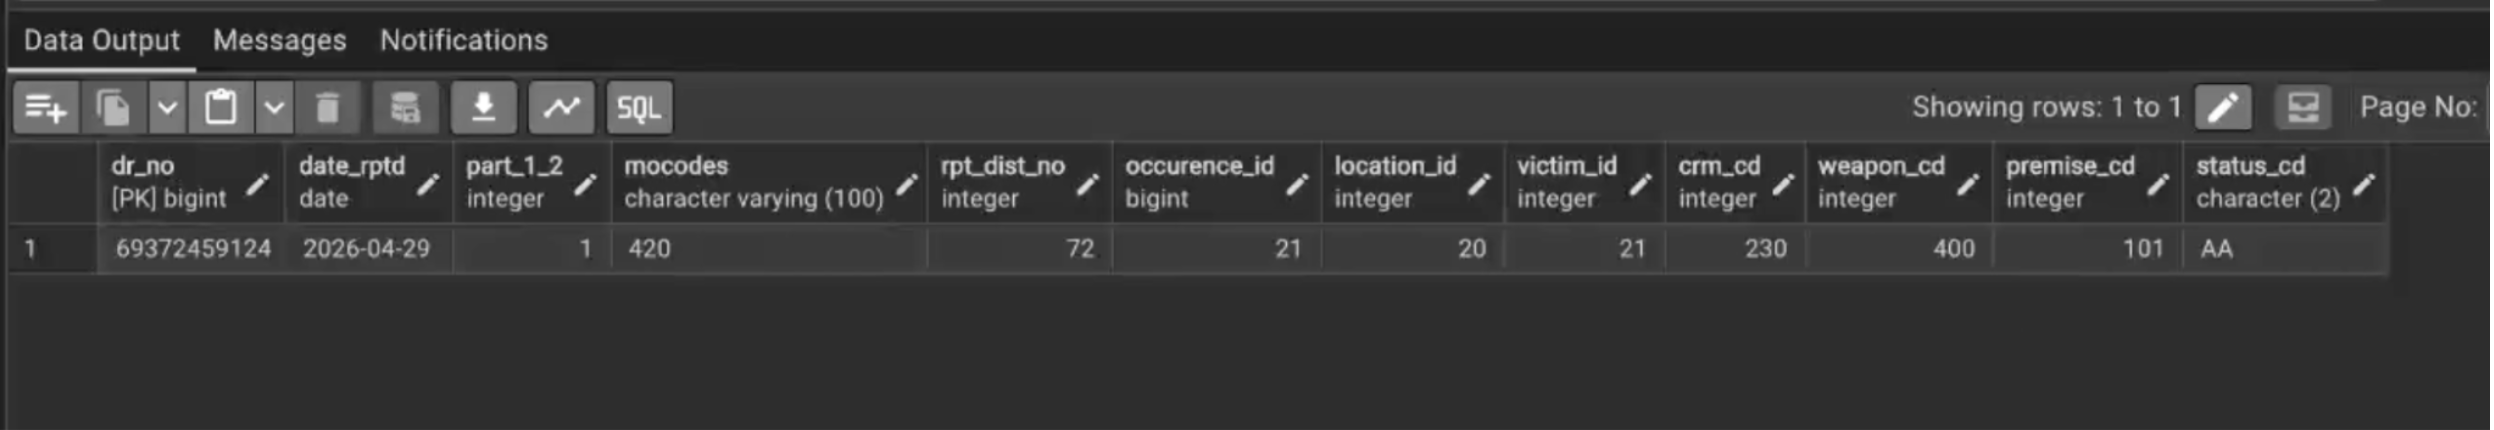
\includegraphics[width=\columnwidth]{procedure-output.png}}
\caption{Output showing the updated Status\_Cd after procedure execution.}
\label{fig:proc_output}
\end{figure}

\subsection{Delete Operation}

The delete operation removes a row from \texttt{Crime\_Report} by its primary key. As shown in Fig.~\ref{fig:delete_query} and Fig.~\ref{fig:delete_output}, after deletion a subsequent select on that primary key returns no results, confirming successful removal.

\begin{figure}[htbp]
\centerline{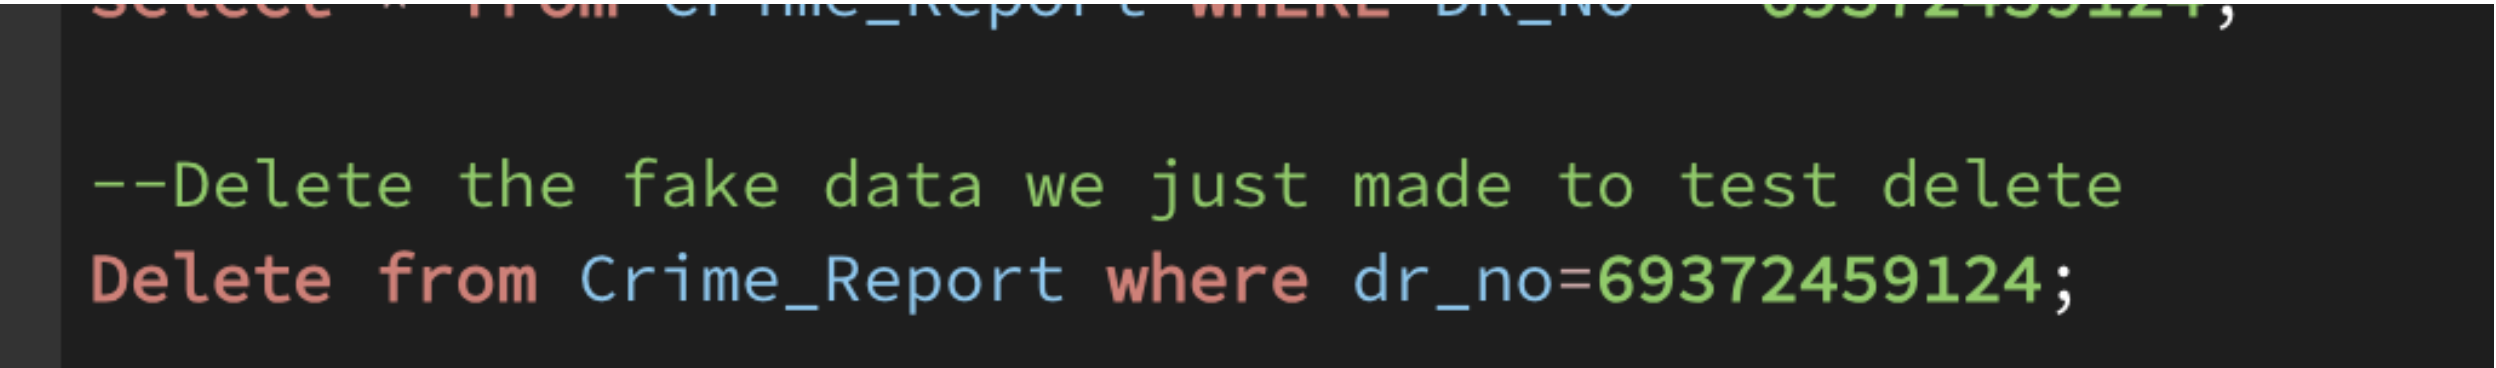
\includegraphics[width=\columnwidth]{delete-query.png}}
\caption{Delete query removing a row from Crime\_Report by primary key.}
\label{fig:delete_query}
\end{figure}

\begin{figure}[htbp]
\centerline{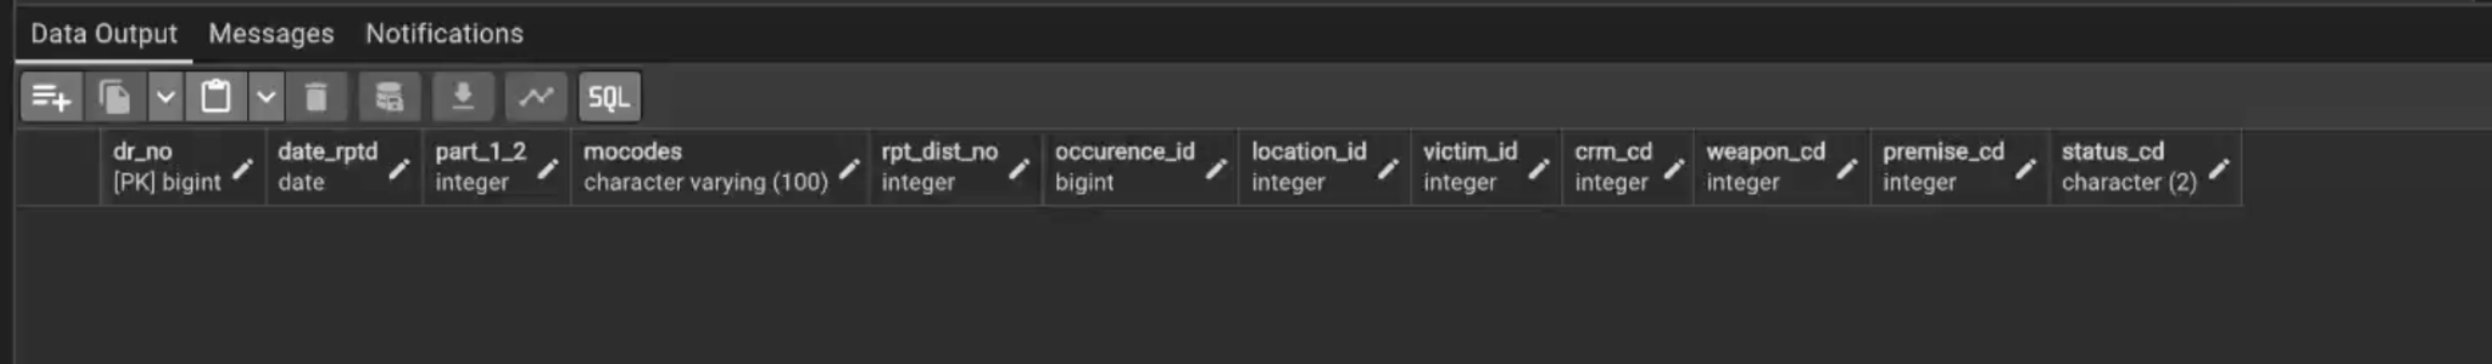
\includegraphics[width=\columnwidth]{delete-output.png}}
\caption{Output confirming the deleted row is no longer present.}
\label{fig:delete_output}
\end{figure}

\subsection{User-Defined Function: Get Crime Count}

The \texttt{get\_crime\_count} function accepts an area name as its input parameter, declares a local \texttt{crime\_count} variable, performs a multi-table join across \texttt{Crime\_Report}, \texttt{Location}, and \texttt{Area}, selects the count of all matching crime reports, stores the result in \texttt{crime\_count}, and returns that integer. Fig.~\ref{fig:func_query} shows the function body, and Fig.~\ref{fig:func_output} shows a sample invocation with its returned value.

\begin{figure}[htbp]
\centerline{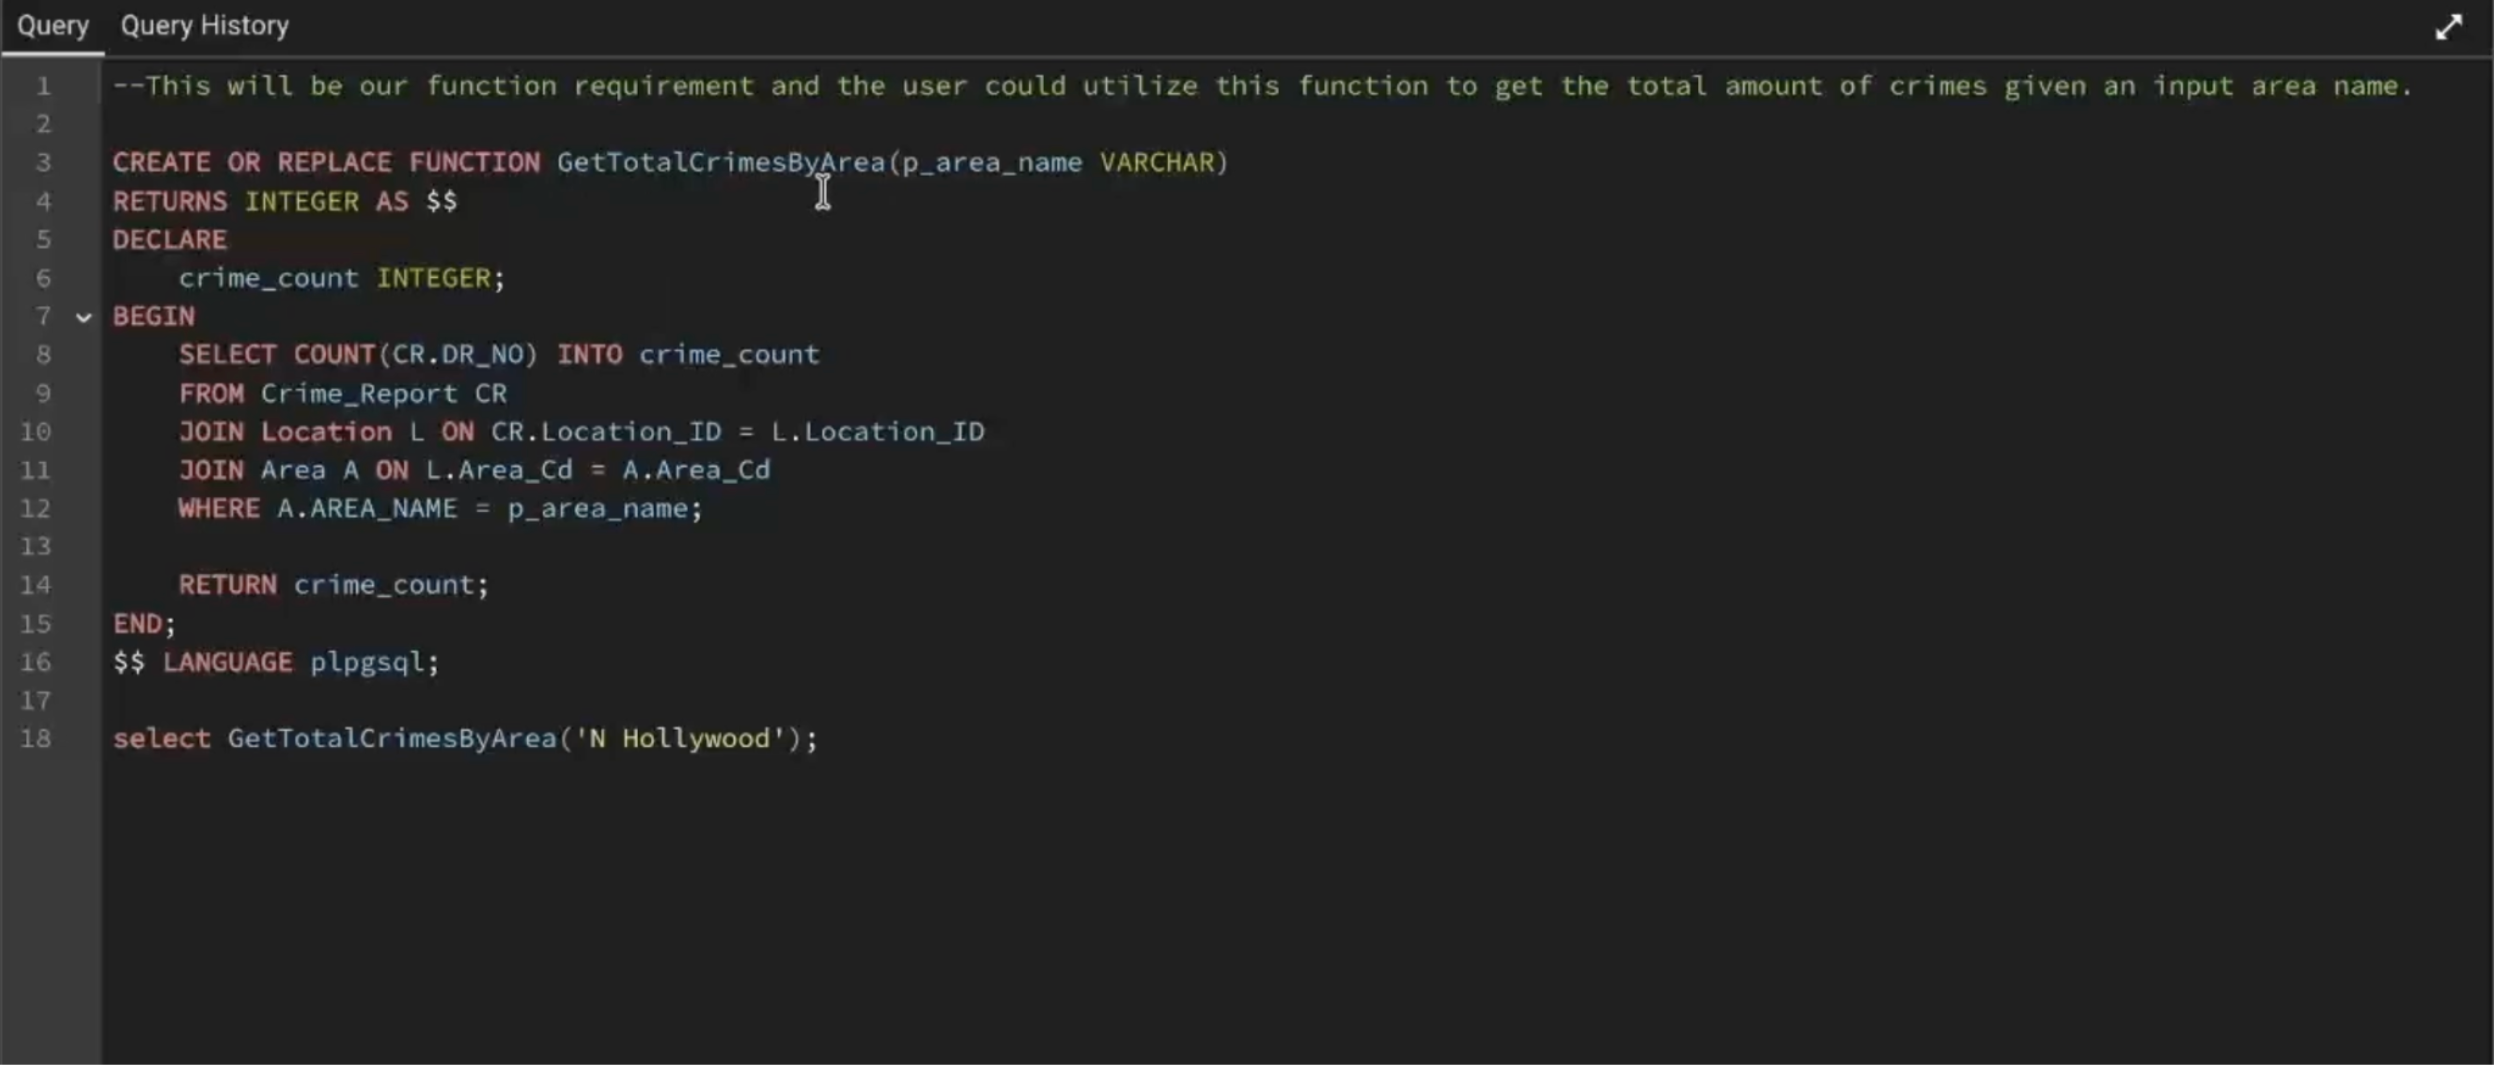
\includegraphics[width=\columnwidth]{get_crime_count_function_query.png}}
\caption{Definition of the get\_crime\_count function.}
\label{fig:func_query}
\end{figure}

\begin{figure}[htbp]
\centerline{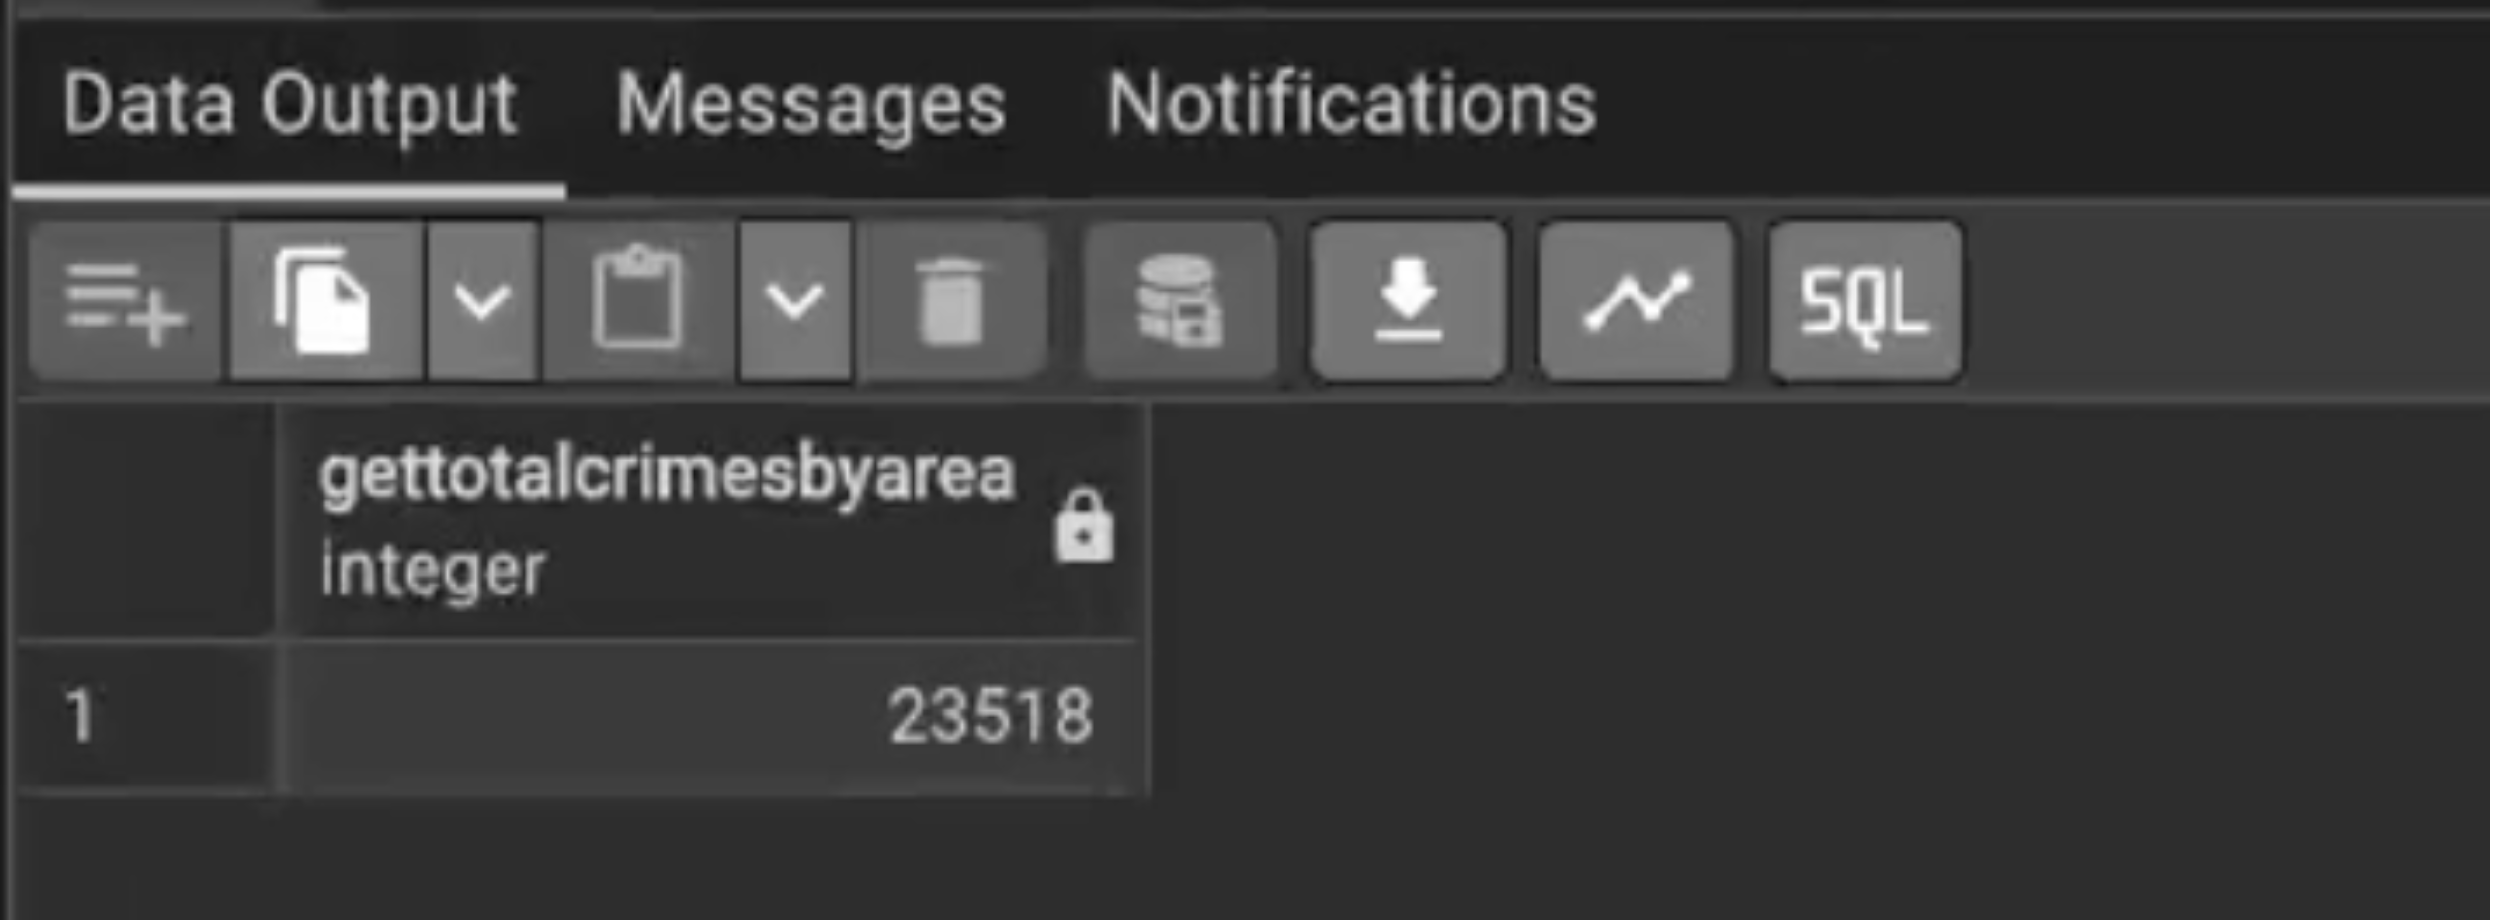
\includegraphics[width=\columnwidth]{get_crime_count_output.png}}
\caption{Sample output of get\_crime\_count returning the total crimes for a given area.}
\label{fig:func_output}
\end{figure}

\subsection{Select Queries}

Four analytical queries demonstrate the database's reporting capabilities.

\subsubsection{Query 1: Five Most Recent Crime Reports}

This query returns the 5 most recent crime reports by occurrence date, including the area name, location name, and crime description. It joins the \texttt{Occurrence}, \texttt{Location}, \texttt{Area}, and \texttt{Crime\_Type} tables, orders results by descending \texttt{DATE\_OCC}, and applies a \texttt{LIMIT 5}. Fig.~\ref{fig:sq1} and Fig.~\ref{fig:sq1_out} show the query and its output.

\begin{figure}[htbp]
\centerline{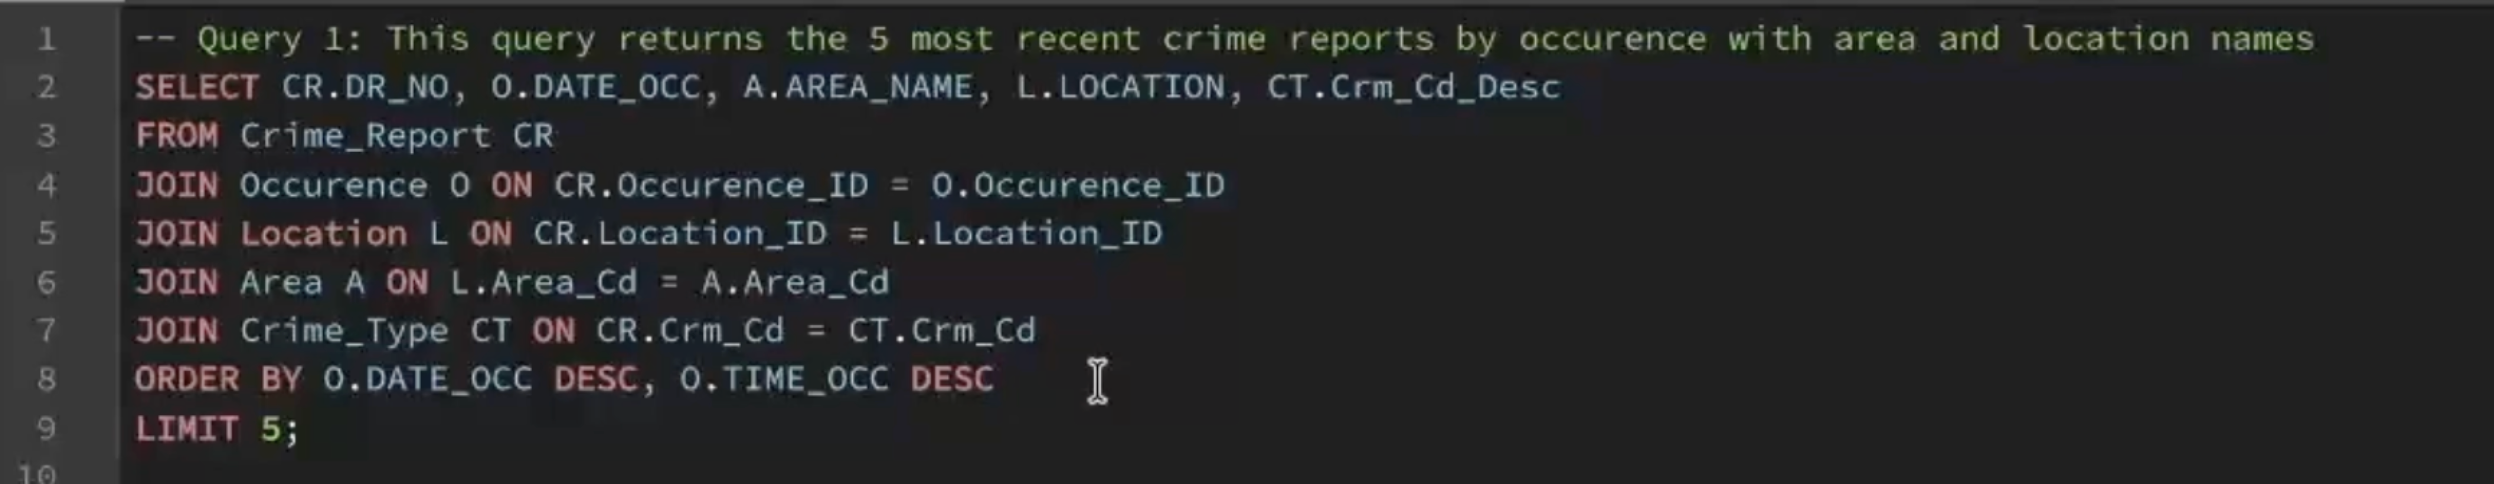
\includegraphics[width=\columnwidth]{select_query1.png}}
\caption{Query 1: Five most recent crime reports with area and location details.}
\label{fig:sq1}
\end{figure}

\begin{figure}[htbp]
\centerline{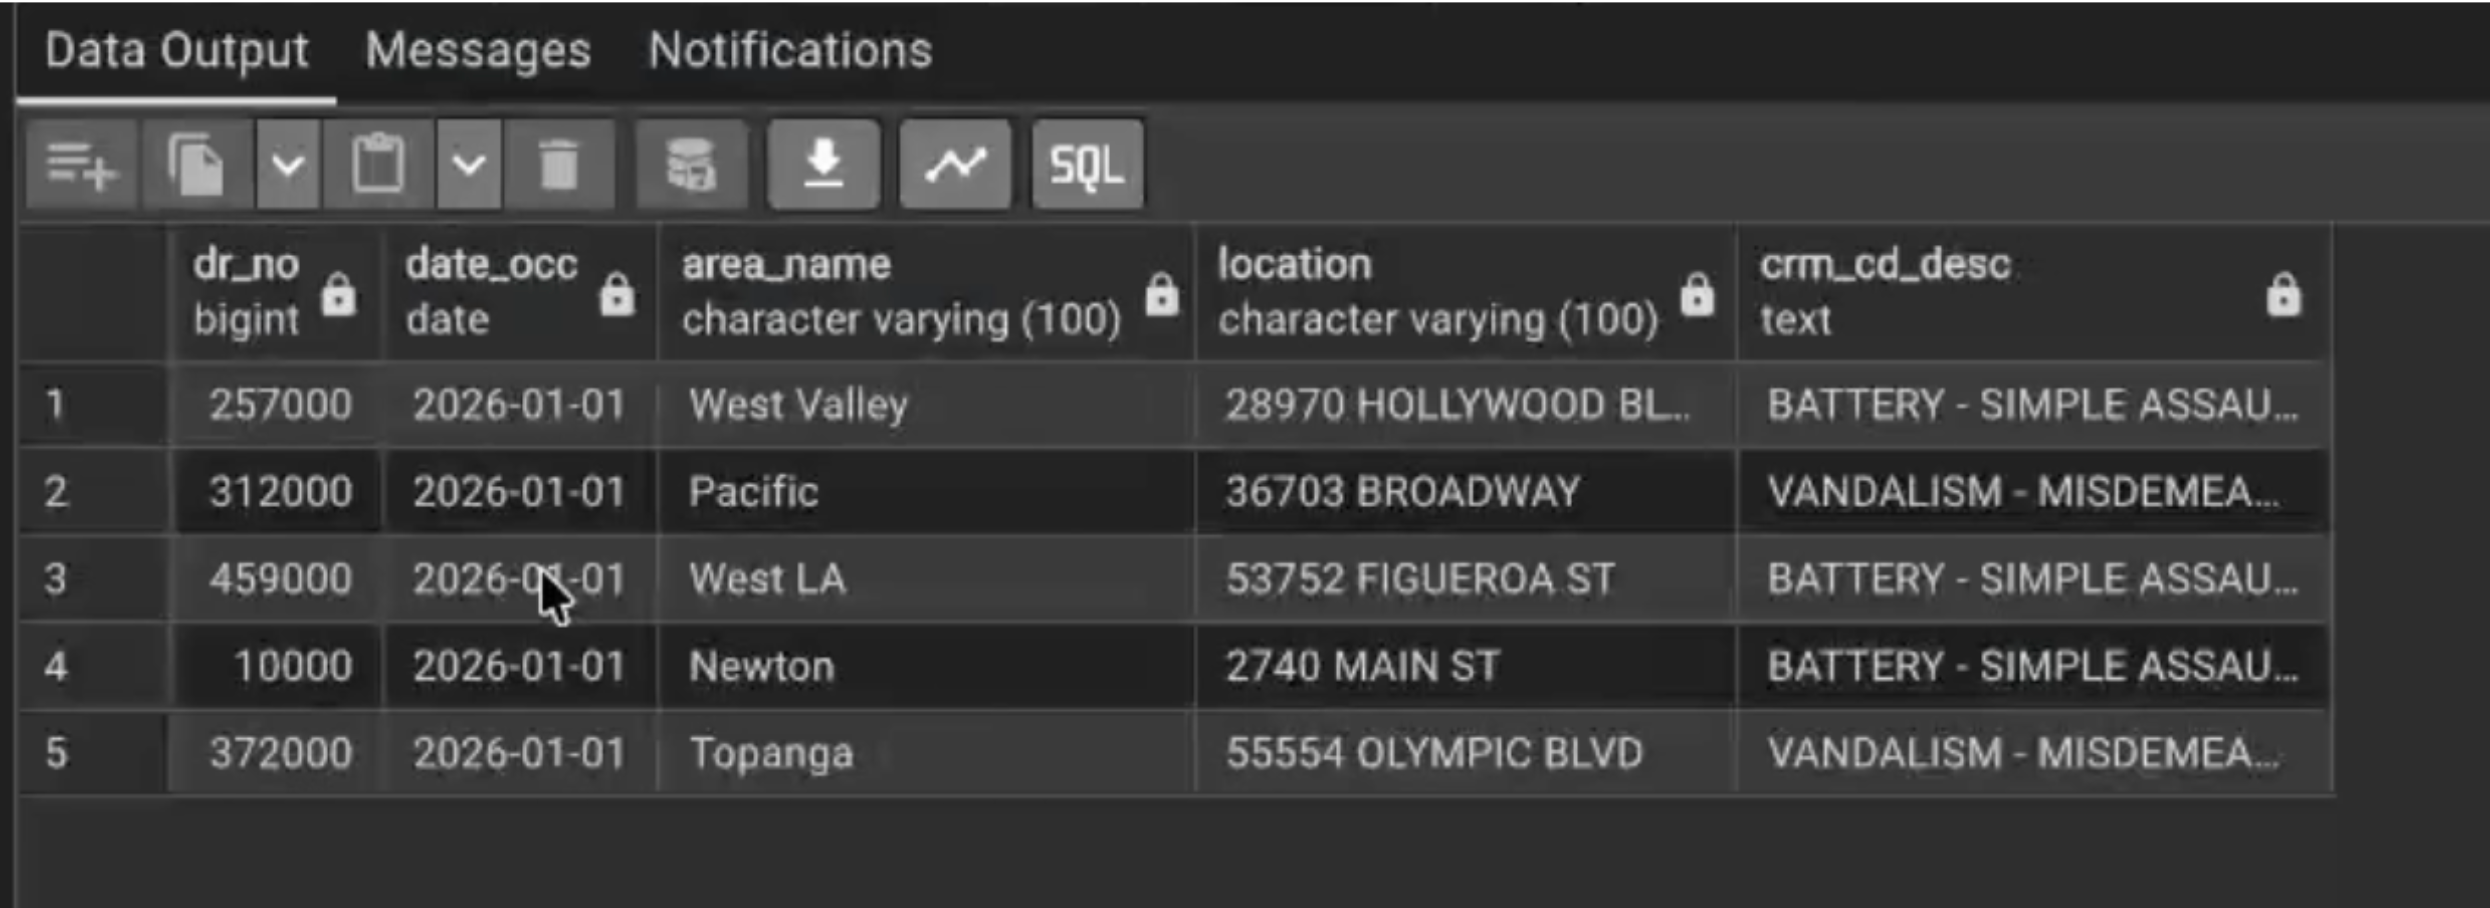
\includegraphics[width=\columnwidth]{select_query1_output.png}}
\caption{Output of Query 1.}
\label{fig:sq1_out}
\end{figure}

\subsubsection{Query 2: High-Crime-Rate Areas}

This query returns the names of all areas with more than 20,000 crime reports, identifying locations with a high crime rate. A subquery aggregates crime counts per area to satisfy the subquery requirement. Fig.~\ref{fig:sq2} and Fig.~\ref{fig:sq2_out} show the query and its output.

\begin{figure}[htbp]
\centerline{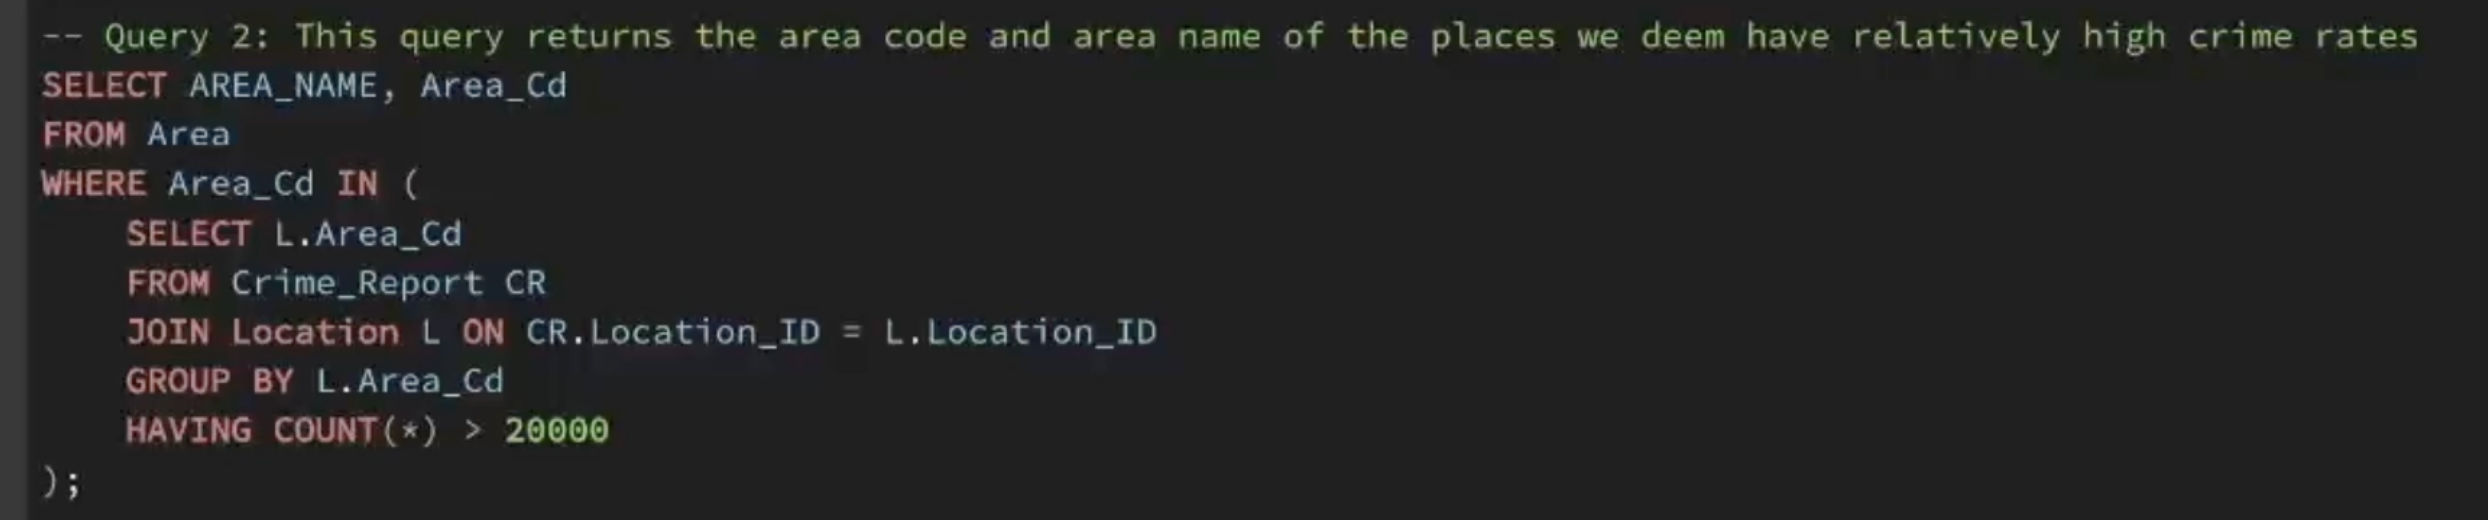
\includegraphics[width=\columnwidth]{select_query_2.png}}
\caption{Query 2: Areas with more than 20,000 crime reports.}
\label{fig:sq2}
\end{figure}

\begin{figure}[htbp]
\centerline{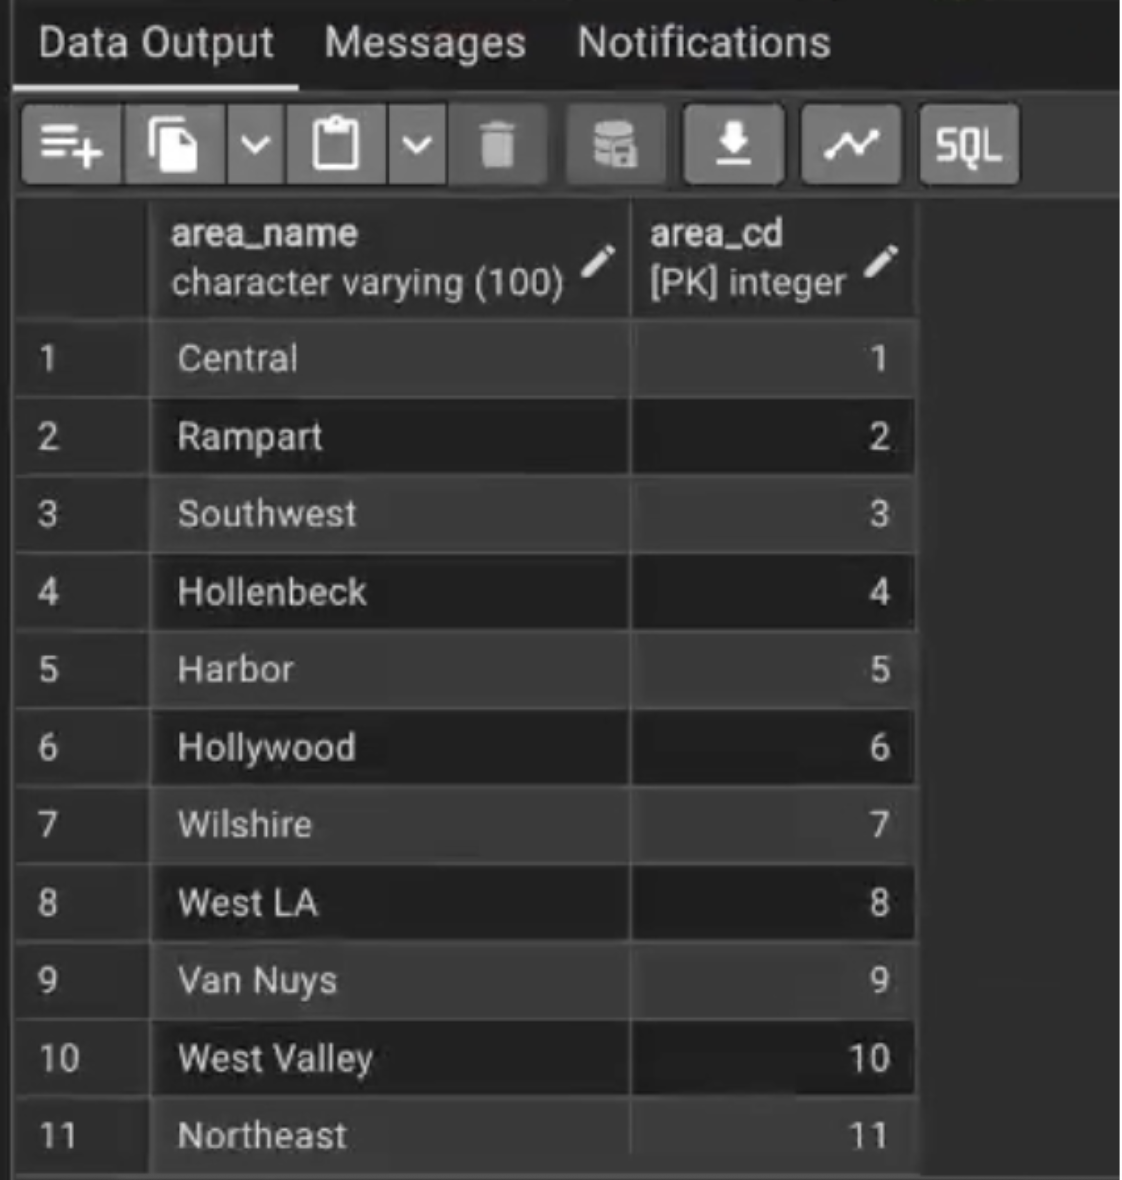
\includegraphics[width=\columnwidth]{select_query_2_output.png}}
\caption{Output of Query 2.}
\label{fig:sq2_out}
\end{figure}

\subsubsection{Query 3: Premises Ordered by Crime Count}

This query returns all premise types ordered by the total number of crimes recorded at each type, providing a ranked view of the most crime-prone venue categories. Fig.~\ref{fig:sq3} and Fig.~\ref{fig:sq3_out} show the query and its output.

\begin{figure}[htbp]
\centerline{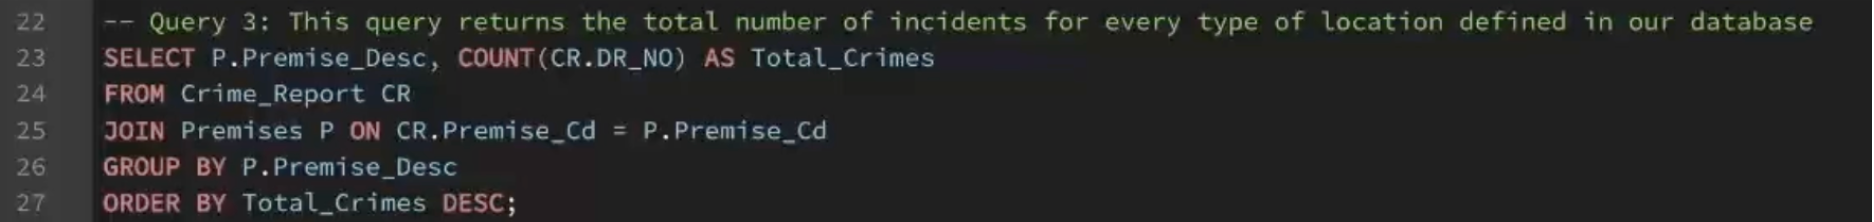
\includegraphics[width=\columnwidth]{select_query_3.png}}
\caption{Query 3: All premise types ordered by total crime count.}
\label{fig:sq3}
\end{figure}

\begin{figure}[htbp]
\centerline{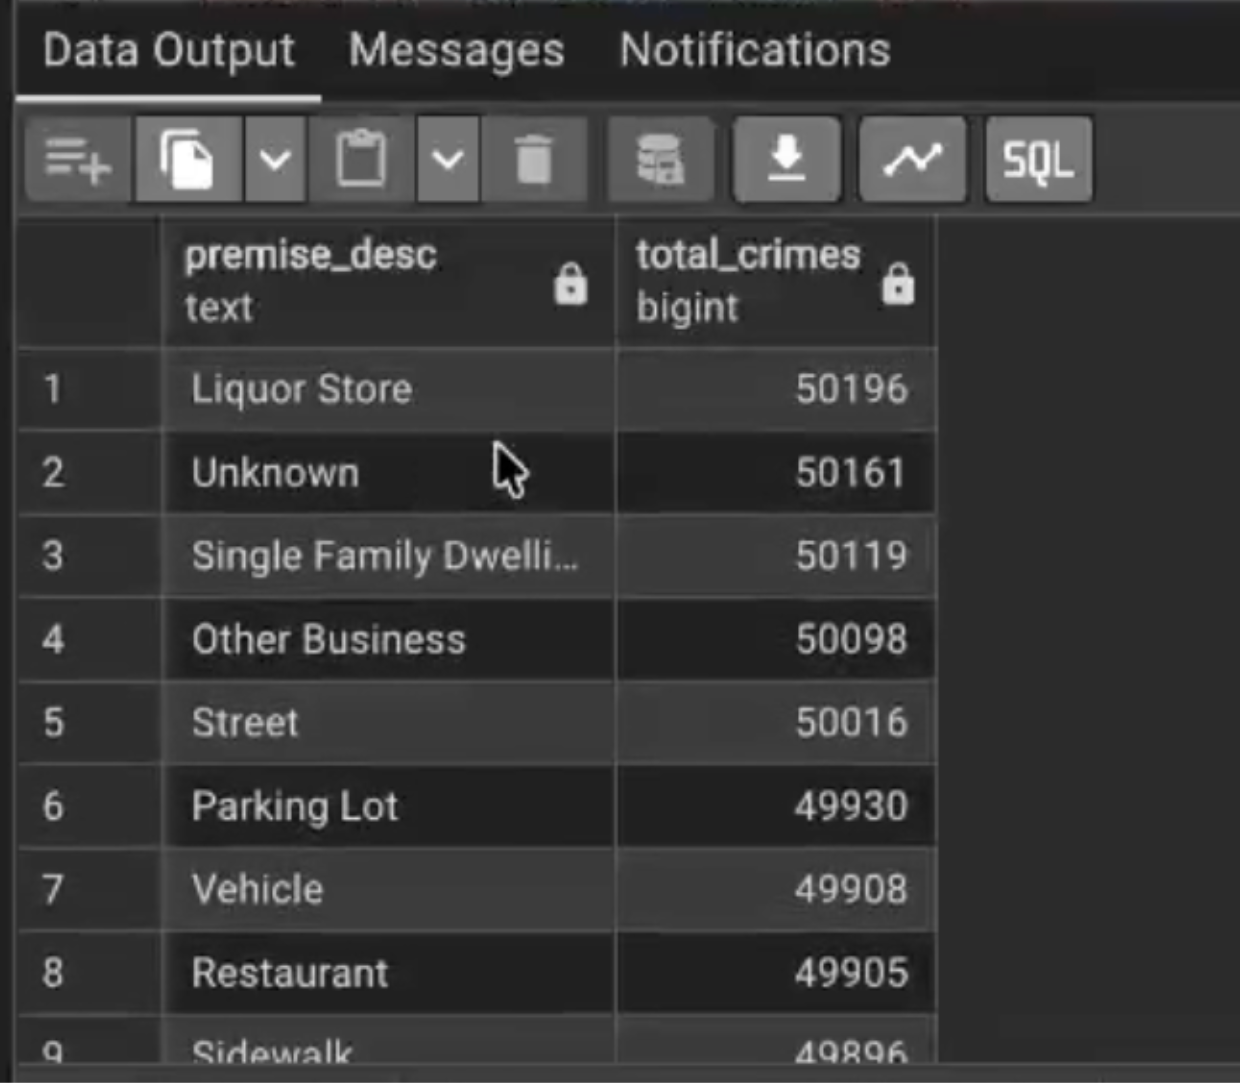
\includegraphics[width=\columnwidth]{select_query_3_output.png}}
\caption{Output of Query 3.}
\label{fig:sq3_out}
\end{figure}

\subsubsection{Query 4: Top 100 Crime-Type and Weapon Combinations}

This query identifies the 100 most frequent pairings of crime type and weapon. It joins the \texttt{Crime\_Type} and \texttt{Weapon\_Type} tables, groups by the crime type description and weapon description, counts co-occurrences with \texttt{COUNT(*)}, and orders by descending incident count. Fig.~\ref{fig:sq4} and Fig.~\ref{fig:sq4_out} show the query and its output.

\begin{figure}[htbp]
\centerline{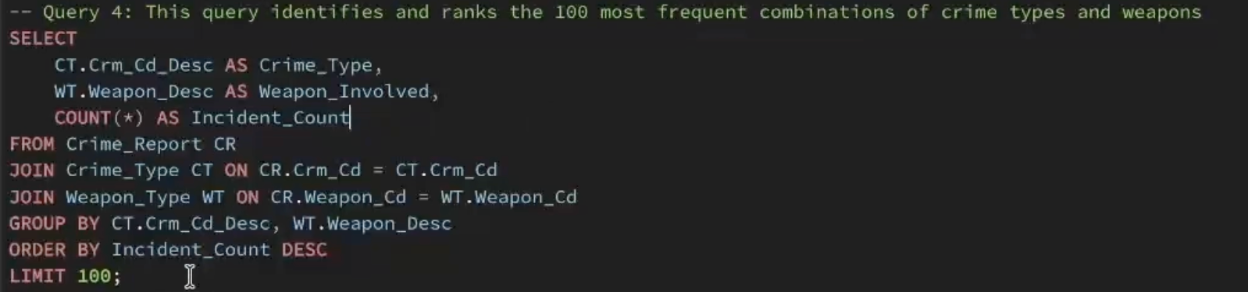
\includegraphics[width=\columnwidth]{select_query_4.png}}
\caption{Query 4: Top 100 most frequent crime-type and weapon combinations.}
\label{fig:sq4}
\end{figure}

\begin{figure}[htbp]
\centerline{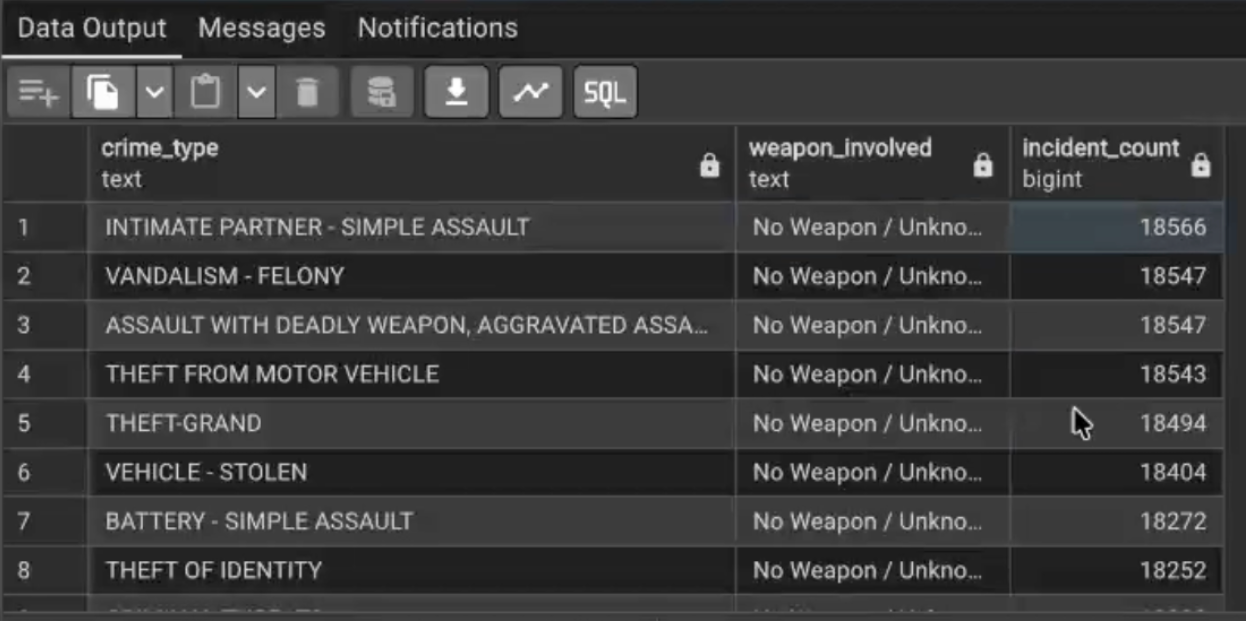
\includegraphics[width=\columnwidth]{select_query_4_output.png}}
\caption{Output of Query 4.}
\label{fig:sq4_out}
\end{figure}

\subsection{Transaction with Trigger Validation}

The transaction file first defines a trigger on the \texttt{Victim\_Type} table that fires on every \texttt{INSERT}. The trigger calls a validation function that checks whether the inserted age value falls between 0 and 120 (inclusive). If the age is outside this range, the function raises an exception, aborting the insert.

A test transaction then attempts to insert two victim records. The first record has a valid age, but the second has an invalid age. Because the second insert raises an exception, the entire transaction rolls back due to atomicity---neither victim record is committed, even though the first insert would have been valid in isolation. This demonstrates correct constraint enforcement through trigger-based validation. Fig.~\ref{fig:trans_query} and Fig.~\ref{fig:trans_output} show the transaction and its output.

\begin{figure}[htbp]
\centerline{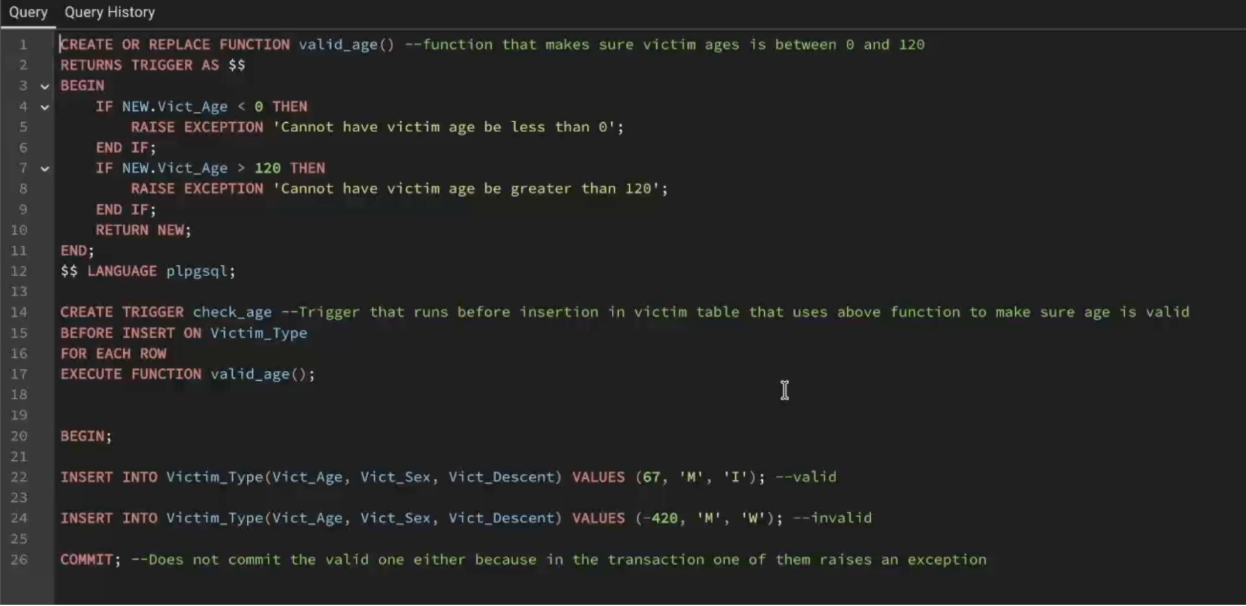
\includegraphics[width=\columnwidth]{transaction_query.png}}
\caption{Transaction query with trigger-based age validation on Victim\_Type inserts.}
\label{fig:trans_query}
\end{figure}

\begin{figure}[htbp]
\centerline{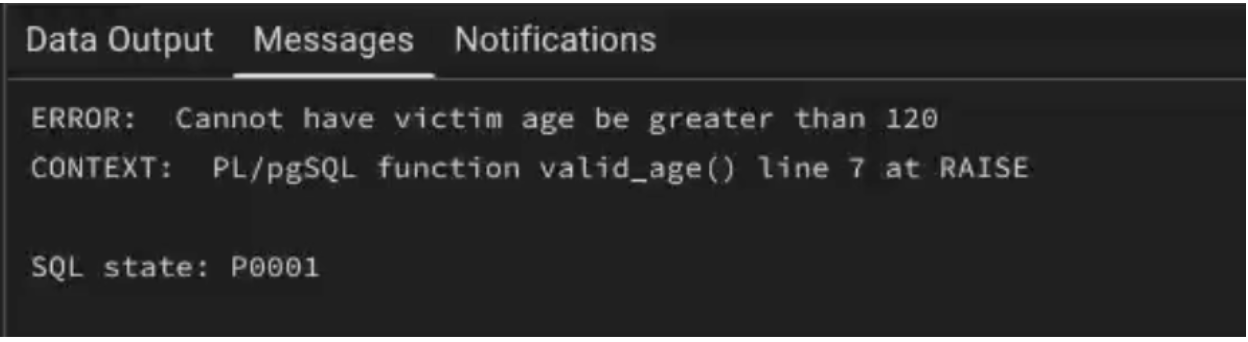
\includegraphics[width=\columnwidth]{transaction_query_output.png}}
\caption{Output showing the full transaction rollback caused by the invalid age value.}
\label{fig:trans_output}
\end{figure}

\subsection{Index Optimization}

Three indexes were created to improve query performance. For each, query execution plans were captured before and after index creation using \texttt{EXPLAIN ANALYZE} to quantify the improvement.

\subsubsection{Index 1}

Fig.~\ref{fig:idx1_query} shows the indexed query definition. Before index creation the planner estimated a cost of approximately 1000.00 (Fig.~\ref{fig:idx1_before}). After index creation, the cost dropped to approximately 6.53 (Fig.~\ref{fig:idx1_after}), a reduction of over 99\%.

\begin{figure}[htbp]
\centerline{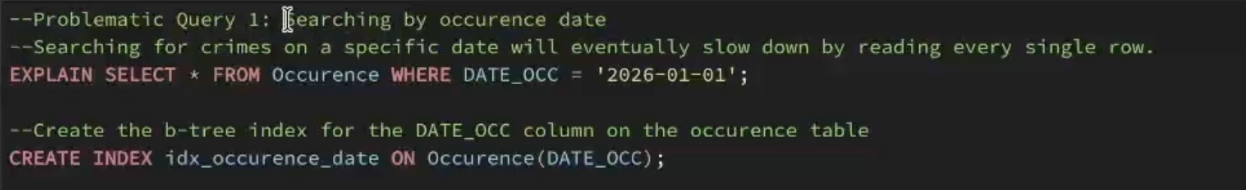
\includegraphics[width=\columnwidth]{index1_query.png}}
\caption{Index 1 query and index definition.}
\label{fig:idx1_query}
\end{figure}

\begin{figure}[htbp]
\centerline{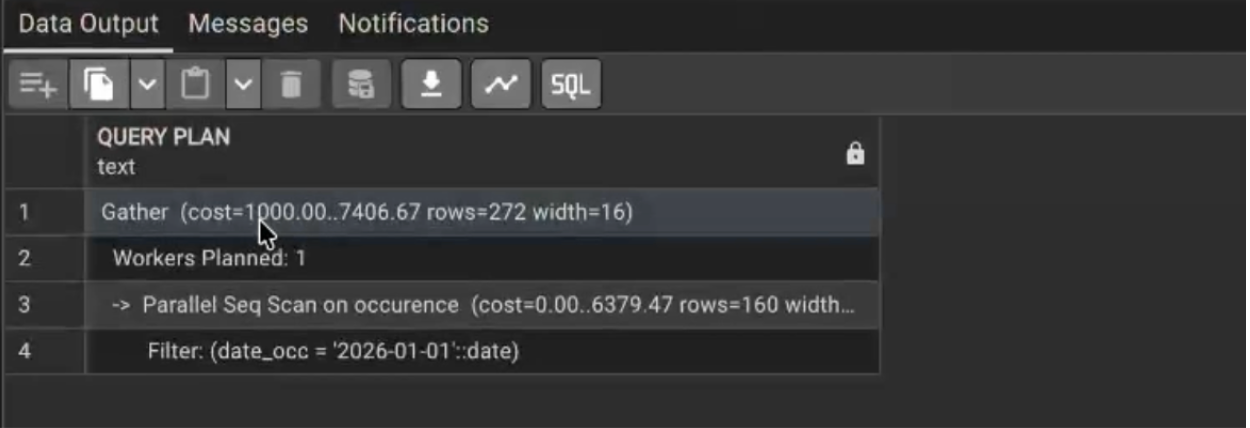
\includegraphics[width=\columnwidth]{index_query_1_before.png}}
\caption{Index 1 execution plan before index creation (cost $\approx$ 1000.00).}
\label{fig:idx1_before}
\end{figure}

\begin{figure}[htbp]
\centerline{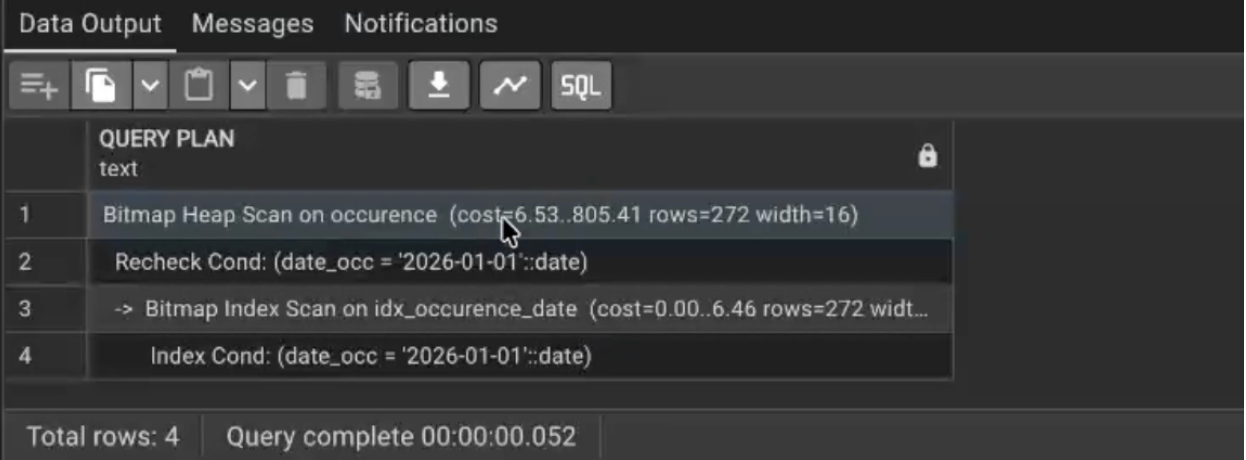
\includegraphics[width=\columnwidth]{index_query_1_after.png}}
\caption{Index 1 execution plan after index creation (cost $\approx$ 6.53).}
\label{fig:idx1_after}
\end{figure}

\subsubsection{Index 2}

Fig.~\ref{fig:idx2_query} shows the second indexed query. The index reduced the cost from approximately 14,175.31 to 13,954.75 (Fig.~\ref{fig:idx2_before} and Fig.~\ref{fig:idx2_after}), representing a modest but measurable improvement for this more complex join-heavy query.

\begin{figure}[htbp]
\centerline{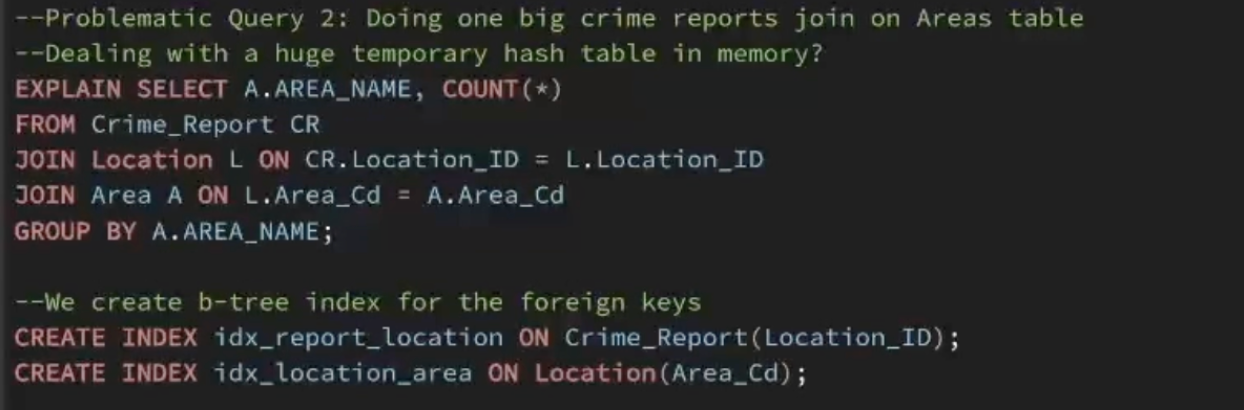
\includegraphics[width=\columnwidth]{index_query_2.png}}
\caption{Index 2 query and index definition.}
\label{fig:idx2_query}
\end{figure}

\begin{figure}[htbp]
\centerline{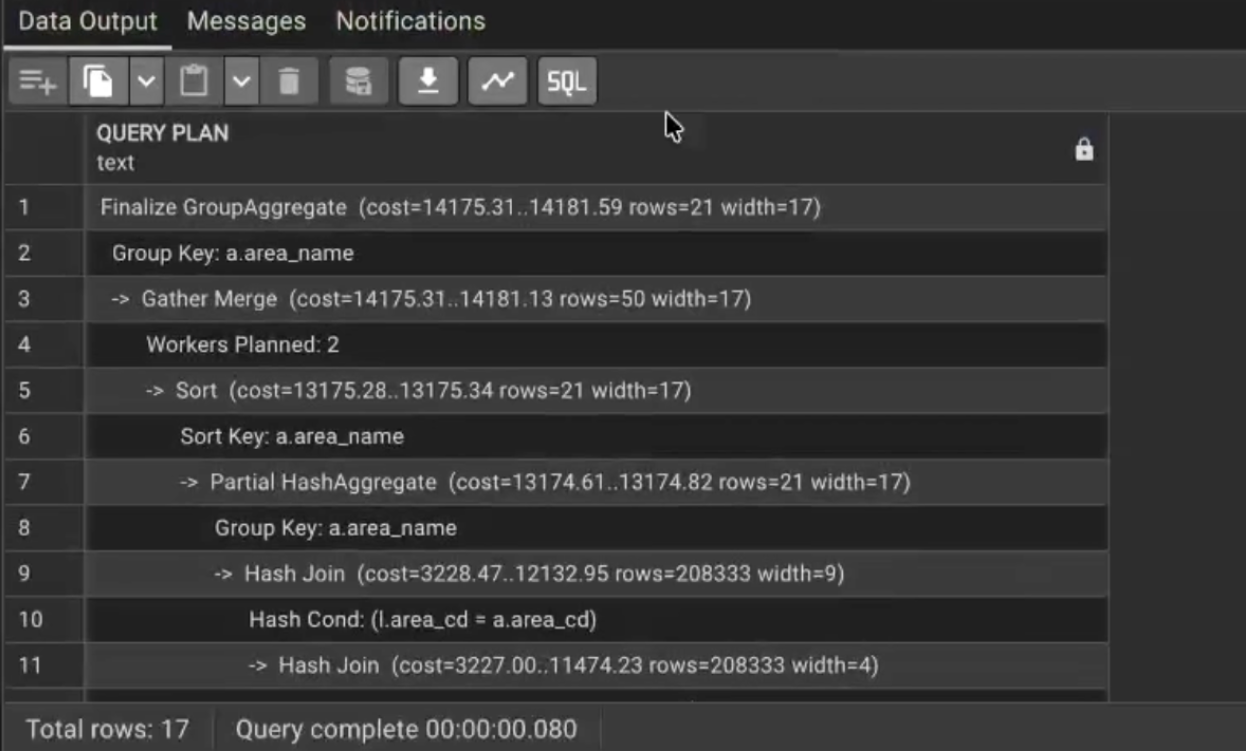
\includegraphics[width=\columnwidth]{index_query_2_before.png}}
\caption{Index 2 execution plan before index creation (cost $\approx$ 14175.31).}
\label{fig:idx2_before}
\end{figure}

\begin{figure}[htbp]
\centerline{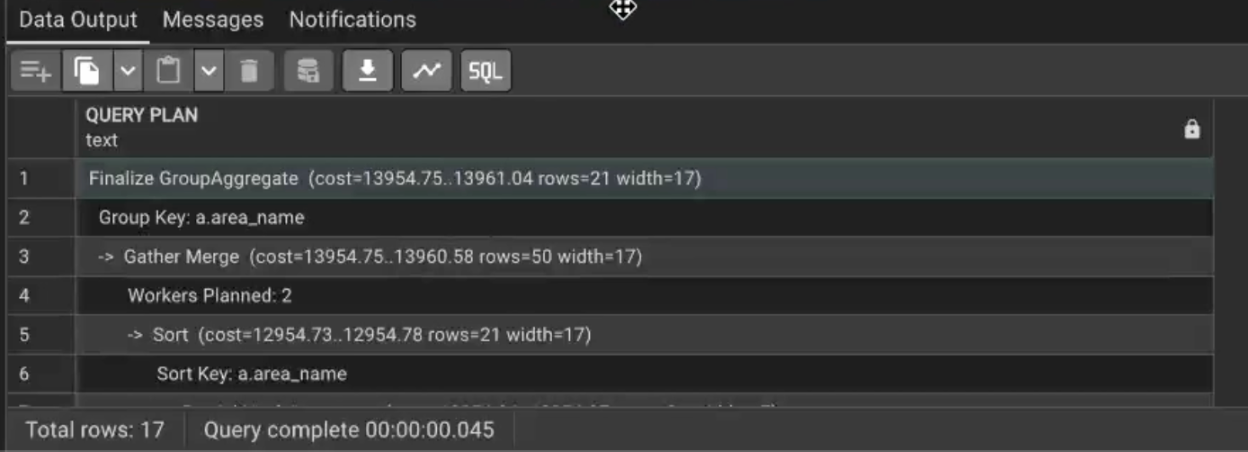
\includegraphics[width=\columnwidth]{index_query_2_after.png}}
\caption{Index 2 execution plan after index creation (cost $\approx$ 13954.75).}
\label{fig:idx2_after}
\end{figure}

\subsubsection{Index 3}

Fig.~\ref{fig:idx3_query} shows the third indexed query. Before index creation the cost was approximately 1000.00; after creation the cost fell to approximately 8.82 (Fig.~\ref{fig:idx3_before} and Fig.~\ref{fig:idx3_after}), again exceeding 99\% cost reduction.

\begin{figure}[htbp]
\centerline{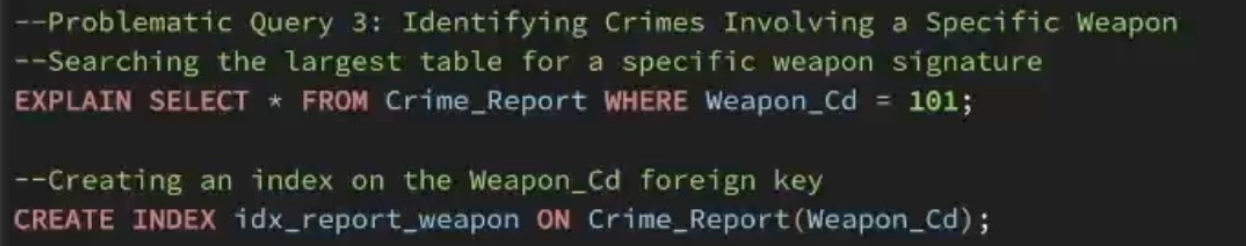
\includegraphics[width=\columnwidth]{index_query_3.png}}
\caption{Index 3 query and index definition.}
\label{fig:idx3_query}
\end{figure}

\begin{figure}[htbp]
\centerline{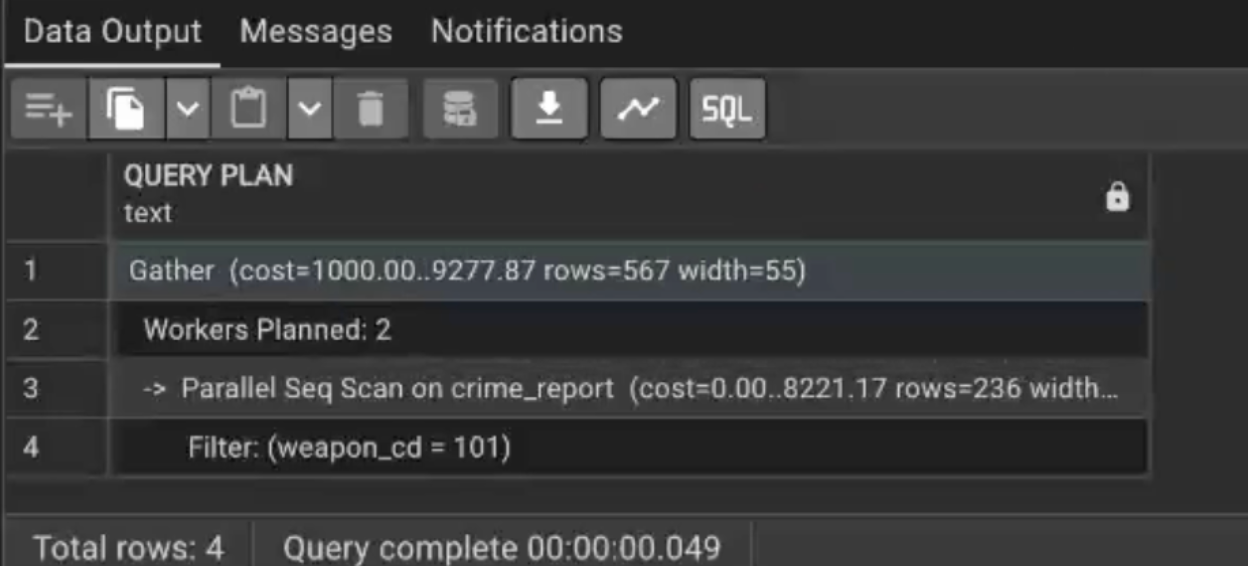
\includegraphics[width=\columnwidth]{index_query_3_before.png}}
\caption{Index 3 execution plan before index creation (cost $\approx$ 1000.00).}
\label{fig:idx3_before}
\end{figure}

\begin{figure}[htbp]
\centerline{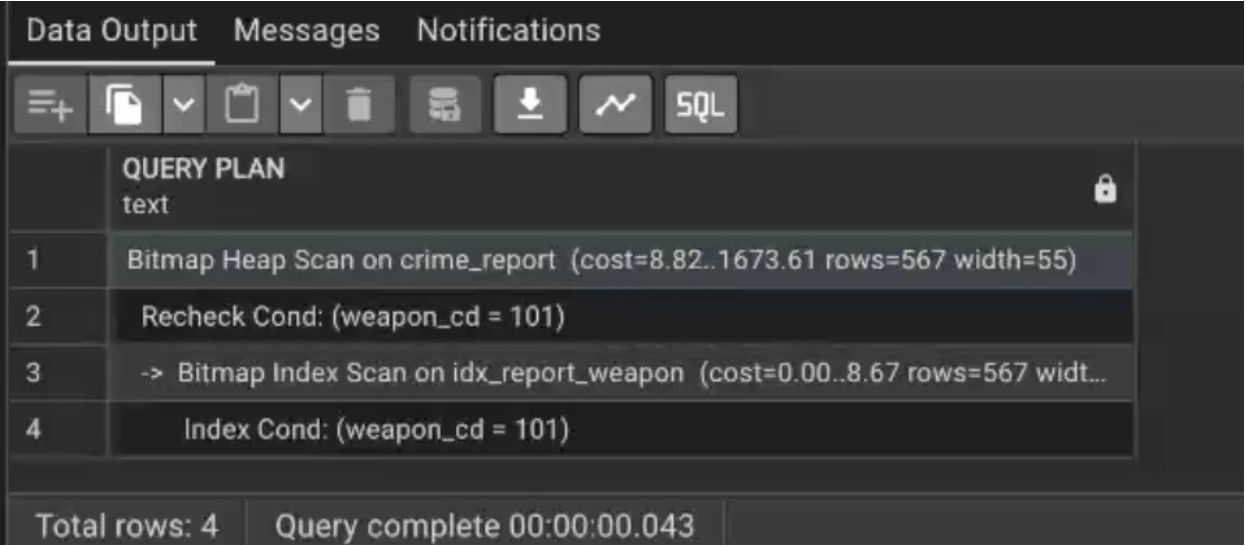
\includegraphics[width=\columnwidth]{index_query_3_after.png}}
\caption{Index 3 execution plan after index creation (cost $\approx$ 8.82).}
\label{fig:idx3_after}
\end{figure}

% ---------------------------------------------------------------
\section{Conclusion}

This paper presented the design and Phase 2 implementation of the LA Crime Analytics database, a normalized relational system that transforms raw LAPD crime data into a structured, queryable resource. The nine-table schema captures all relevant facets of crime reports: occurrence timing, geographic location, victim demographics, crime classification, weapon type, premise type, and case status. Enforced normalization ensures data consistency and eliminates redundancy across the hundreds of thousands of records in the dataset.

Phase 2 demonstrated the database's practical value through data modification scripts, a status-update stored procedure, a per-area crime count function, four analytical queries covering recency, high-crime areas, premise rankings, and crime-weapon co-occurrence, a transactional trigger that enforces victim age constraints via atomicity, and three index optimizations that achieved cost reductions exceeding 99\% in two of three scenarios.

The LA Crime Analytics schema provides a replicable blueprint that other cities could adopt to enable data-driven crime analysis, supporting residents, law enforcement agencies, and city governments in making informed, evidence-based decisions.

% ---------------------------------------------------------------
\section*{Acknowledgment}

The authors thank the Los Angeles Police Department for making the crime dataset publicly available through the Los Angeles Open Data Portal. The E/R diagram was created using Lucidchart.

\begin{thebibliography}{00}
\bibitem{lapd} Los Angeles Police Department, ``Crime Data from 2020 to Present,'' \textit{Los Angeles Open Data Portal}. [Online]. Available: https://data.lacity.org/Public-Safety/Crime-Data-from-2020-to-Present/2nrs-mtv8

\bibitem{lucidchart} Lucid Software Inc., ``Lucidchart Diagramming Application,'' 2024. [Online]. Available: https://lucid.app/
\end{thebibliography}

\end{document}
